\documentclass[11pt]{amsart}
\usepackage[margin=1.15in]{geometry}
\usepackage{amssymb,amsmath,mathtools}
\usepackage{graphicx,booktabs,array,float}
\usepackage[hidelinks]{hyperref}
\usepackage[expansion=false]{microtype}

\newtheorem{theorem}{Theorem}[section]
\newtheorem{proposition}[theorem]{Proposition}
\newtheorem{lemma}[theorem]{Lemma}
\newtheorem{corollary}[theorem]{Corollary}
\newtheorem{mainthm}{Theorem}
\renewcommand{\themainthm}{\Alph{mainthm}}
\theoremstyle{definition}
\newtheorem{definition}[theorem]{Definition}
\newtheorem{remark}[theorem]{Remark}
\newtheorem{example}[theorem]{Example}

\newcommand{\ZZ}{\mathbb{Z}}
\newcommand{\cc}{\hat c}
\newcommand{\dt}{\tilde d}
\newcommand{\vt}{\vartheta}
\newcommand{\Kzero}{90}
\newcommand{\zenodoCodeDOI}{10.5281/zenodo.XXXXXXX}

\setlength{\emergencystretch}{2.5em}
\hbadness=2000
\raggedbottom
\begin{document}

\title[Black hole indices of $\mathcal N=8$ string theory are positive]{Black Hole Indices of $\mathcal{N}=8$\\ String Theory Are Positive}

\author{Deep Bhattacharjee}
\address{Formerly, Electro-Gravitational Space Propulsion Laboratory (EGSPL), Bhubaneswar, Odisha 751030, India}
\address{Formerly, University of Calcutta (Heramba Chandra College), 23/49 Gariahat Road, Golpark, Kolkata 700029, West Bengal, India}
\email{d.bhattacharjee@erl-forschung.de}
\email{itsdeep@live.com}
\email{egspl@proton.me (GitHub-related contact; GitHub account creelie)}
\urladdr{https://orcid.org/0000-0003-0466-750X}

\begin{abstract}
Sen predicted that the protected indices of single-centred black holes in type~II string theory on $T^6$ and $T^5$ are positive. We prove this for every charge whose index is known: four-dimensional dyons, five-dimensional rotating black holes, and five-dimensional black holes of fixed angular momentum.

\medskip\noindent\textbf{Keywords:} black hole microstates; helicity trace index; Jacobi forms.

\smallskip\noindent\textbf{MSC 2020:} 11F50 (primary); 11P82, 81T30, 83E30.
\end{abstract}

\maketitle

\section{Introduction}\label{sec:intro}

The entropy of a supersymmetric black hole in string theory can be compared with a count of microscopic states. Strominger and Vafa did this for five-dimensional black holes made of D1- and D5-branes with momentum \cite{SV96}, Breckenridge, Myers, Peet and Vafa added angular momentum \cite{BMPV97}, and Maldacena, Moore and Strominger found the exact count for type~II string theory on a torus \cite{MMS99}. In four dimensions the analogous formula was derived by Shih, Strominger and Yin from the relation between four- and five-dimensional black holes \cite{GSY06,SSY06}, and Sen extended it to all charges of a certain primitivity type \cite{Sen08b,Sen10}. These formulae count the states with a sign: what is computed at weak coupling is a helicity trace index, the quantity that does not change when the coupling is increased until the black hole forms \cite{BK97,BFKOV98,KO97,Sen08r}.

A black hole is more than the integer that counts it. Sen observed that a single-centred black hole whose only hair outside the horizon are the zero modes of the broken supersymmetries has a horizon of zero angular momentum, so that its microstates all contribute to the index with the same sign. Once the zero modes are removed, the index must therefore be a positive integer \cite{Sen11,DGMS11,CGMS16}. For the black holes of type~II string theory on $T^6$ the multi-centred configurations that could spoil this do not contribute \cite{Sen08b,Sen10}, so the prediction applies to the microscopic formula itself. It is a nontrivial statement about Fourier coefficients: the formulae are sums of coefficients of the Jacobi form $\phi_{-2,1}$, whose signs alternate.\footnote{For $\mathcal N=4$ string theory the corresponding prediction concerns Siegel modular forms, and positivity holds there only after wall crossing is taken into account \cite{Sen11}. The $\mathcal N=8$ case is simpler in that the index is a finite divisor sum, but it is not a single coefficient.} Bringmann and Murthy stated the prediction for the four- and five-dimensional black holes of type~II on $T^6$ and $T^5$ and proved it when the index is a single Fourier coefficient \cite{BM13}. Sen introduced the five-dimensional index at fixed angular momentum \cite{Sen12}, which the same argument predicts to be positive \cite{BM13}.

This paper proves the prediction in full, for every charge for which the index is known.

\subsection*{The indices}
Write $q=e^{2\pi i\tau}$ and $\zeta=e^{2\pi iz}$, and define the integers $\cc(D)$ by
\begin{equation}\label{eq:phi}
-\frac{\vt_1(\tau,z)^2}{\eta(\tau)^6}=\sum_{k,l\in\ZZ}\cc(4k-l^2)\,q^k\zeta^l ,
\end{equation}
so that $\cc(-1)=1$, $\cc(0)=-2$, $\cc(3)=8$, $\cc(4)=-12$, $\cc(7)=39$, $\cc(8)=-56$, and $\cc(D)=0$ when $D<-1$ or $D\equiv1,2\pmod 4$. The left side is the weak Jacobi form $\phi_{-2,1}$ of weight $-2$ and index $1$ \cite[\S9]{EZ85}; Section~\ref{sec:background} explains why a coefficient depends only on $4k-l^2$.

In type~IIB on $T^4\times S^1\times\widetilde S^1$, consider D1-, D3- and D5-branes wrapped on $\widetilde S^1$ with charge vector $Q$ and on $S^1$ with charge vector $P$; both lie in the even lattice of signature $(4,4)$ formed by the even homology of $T^4$, and $Q^2$, $P^2$, $Q\cdot P$ are the intersection products \cite{Sen10}. Put
\[
\Delta=Q^2P^2-(Q\cdot P)^2,\qquad \ell_1=\gcd_{i<j}\{Q_iP_j-Q_jP_i\},\qquad \ell_2=\gcd\bigl(\tfrac12Q^2,\tfrac12P^2,Q\cdot P\bigr).
\]
A black hole with these charges exists when $\Delta>0$; its entropy is $\pi\sqrt\Delta$ \cite{KK96}. When $\gcd(\ell_1,\ell_2)=1$ the index of the states with charges $(Q,P)$ is \cite[(2.4)]{Sen10}\footnote{Sen derives \eqref{eq:d4} from the counting formula of Maldacena, Moore and Strominger \cite{MMS99} and of Shih, Strominger and Yin \cite{SSY06} by a duality transformation to a normal form \cite[\S2, App.~A]{Sen10}; the condition $\gcd(\ell_1,\ell_2)=1$ is what that transformation needs. The integer $d$ is $-B_{14}$, the fourteenth helicity trace with the contribution of the fermion zero modes removed (Section~\ref{ssec:helicity}). Chowdhury, Garavuso, Mondal and Sen recovered the first coefficients of \eqref{eq:d4} by counting the solutions of the supersymmetric vacuum equations of D-brane systems \cite{CGMS14}, and Chowdhury and Maji extended the count \cite{CM24}.}
\begin{equation}\label{eq:d4}
d(Q,P)=(-1)^{Q\cdot P+1}\sum_{s\mid \ell_1\ell_2}s\,\cc\bigl(\Delta/s^2\bigr).
\end{equation}

In type~IIB on $T^4\times S^1$, a system of $Q_1$ D1-branes and $Q_5$ D5-branes with $n$ units of momentum along $S^1$ and angular momentum $J_{3L}=J/2$ forms a rotating five-dimensional black hole when $4Q_1Q_5n-J^2>0$; its entropy is $\pi\sqrt{4Q_1Q_5n-J^2}$ \cite{BMPV97}. Put $M=Q_1Q_5n$ and, for $l\in\ZZ$,
\begin{equation}\label{eq:F}
F(l)=\sum_{s\mid \gcd(n,\,Q_1Q_5,\,l)}s\,\cc\Bigl(\frac{4M-l^2}{s^2}\Bigr).
\end{equation}
For $\gcd(Q_1,Q_5)=1$ the index with fixed $J$ and summed over $\vec J^{\,2}$ is \cite[(5.37)]{DGMS11}, \cite[(5.28)--(5.29)]{Sen12}
\begin{equation}\label{eq:d5}
\dt(n,Q_1,Q_5,J)=(-1)^{J+1}\sum_{r=-2}^{2}(-1)^r\binom{4}{2-r}F(J-r),
\end{equation}
that is, $\sum_J(-1)^{J+1}\dt(J)\zeta^J=(\zeta^{1/2}-\zeta^{-1/2})^4\sum_lF(l)\zeta^l$; the factor $(\zeta^{1/2}-\zeta^{-1/2})^4$ removes the fermion zero modes of the D1-D5 system that carry $J_{3L}$.\footnote{Equation \eqref{eq:d5} is \cite[(5.29)]{Sen12} with the complete divisor sum of \cite[(5.37)]{DGMS11}, in which $Q_1$ is replaced by $Q_1Q_5$. We keep the overall sign of \cite[(5.28)--(5.30)]{Sen12}, in which the prediction reads $\dt>0$ and $d>0$; the index of \cite[(5.37)]{DGMS11}, defined with the extra factor $(-1)^J$ of \cite{MMS99}, is $-\dt$. The sum in \eqref{eq:F} runs over all $s$, including those for which $(4M-l^2)/s^2=-1$; these terms matter in Section~\ref{sec:5d}.} Sen's index at fixed $J$ and fixed $\vec J_L^{\,2}=\tfrac J2(\tfrac J2+1)$ is \cite[(5.30)]{Sen12}
\begin{equation}\label{eq:drot}
d(n,Q_1,Q_5,J)=\dt(n,Q_1,Q_5,J)-\dt(n,Q_1,Q_5,J+2),\qquad J\ge0 .
\end{equation}

\subsection*{Results}
\begin{mainthm}\label{thm:A}
Let $(Q,P)$ be charges with $\Delta>0$ and $\gcd(\ell_1,\ell_2)=1$. Then $d(Q,P)>\tfrac12|\cc(\Delta)|>0$.
\end{mainthm}

\begin{mainthm}\label{thm:B}
Let $Q_1,Q_5,n\ge1$ with $\gcd(Q_1,Q_5)=1$, and $J\in\ZZ$ with $4Q_1Q_5n-J^2>0$. Then $\dt(n,Q_1,Q_5,J)>0$.
\end{mainthm}

\begin{mainthm}\label{thm:C}
Under the hypotheses of Theorem~\ref{thm:B} with $J\ge0$, $d(n,Q_1,Q_5,J)>0$.
\end{mainthm}

The three statements are exactly the predictions of \cite[\S5]{BM13} and \cite[(5.30)]{Sen12}. They cover every charge for which an exact formula is known; the four-dimensional charges with $\gcd(\ell_1,\ell_2)>1$ remain outside, see Section~\ref{ssec:torsion}.

\subsection*{What the proof has to overcome}
The sign of $\cc(D)$ is $(-1)^{D+1}$ (Lemma~\ref{lem:theta}), and $\Delta\equiv Q\cdot P\pmod 2$ because the lattice is even. So the term $s=1$ of \eqref{eq:d4} is $|\cc(\Delta)|$. If $s$ is odd then $s^2\equiv1\pmod 8$ and $\Delta/s^2\equiv\Delta\pmod 2$, so every odd $s$ contributes a positive term as well; this is the observation behind the proofs of \cite{BM13}. An even $s$ breaks it. Take $\tfrac12Q^2=\tfrac12P^2=2$ and $Q\cdot P=2$, for instance $Q=e_1+2f_1$ and $P=e_2+2f_2+2f_1$ in two hyperbolic planes with $e_i\cdot f_i=1$. Then $\ell_1=1$, $\ell_2=2$, $\Delta=12$, and
\[
d(Q,P)=-\bigl(\cc(12)+2\,\cc(3)\bigr)=208-16=192 .
\]
The term $s=2$ is negative. Positivity is then a matter of size: the negative terms must be smaller than the positive ones, for every $\Delta$ and every $\ell_1\ell_2$. In five dimensions the same problem appears in three places: in the divisor sum; in the difference \eqref{eq:drot}, where two coefficients of the same sign are subtracted from each other; and at the values of $l$ with $4M-l^2<0$, where the term $(4M-l^2)/s^2=-1$ of \eqref{eq:F} survives and can carry either sign.

\subsection*{Plan}
The proof rests on one inequality, Proposition~\ref{prop:key}: the growth $|\cc(D)|-|\cc(D-4)|$ of the coefficients within a residue class exceeds twice every divisor sum $\sum_{s\ge2}s^2|\cc(E/s^2)|$ with $E\le D$. Section~\ref{sec:background} collects the background and derives the facts about helicity traces, charge invariants and $\phi_{-2,1}$ that the proof uses. Section~\ref{sec:c} writes $|\cc(D)|$ through the numbers $a(n)$ of partitions of $n$ into parts of six colours; this gives monotonicity and an upper bound. Section~\ref{sec:a} proves explicit bounds for $a(n)$ from above and below. Section~\ref{sec:key} proves the inequality, analytically for $D\ge 359$ and by finite arithmetic below. Sections~\ref{sec:4d} and~\ref{sec:5d} prove the three theorems and work out examples. Section~\ref{sec:remarks} discusses sharpness, the U-duality invariant extension of \cite{MMS99} and the charges not covered by \eqref{eq:d4}. Appendix~\ref{app:standard} derives the elementary facts used along the way, and Appendix~\ref{app:finite} describes the finite computation.

\section{Background}\label{sec:background}

\subsection{Helicity traces and fermion zero modes}\label{ssec:helicity}
Let $h$ be the helicity, the eigenvalue of the rotation generator $J_3$ in the rest frame of a massive particle in four dimensions. The helicity traces are
\[
B_{2m}=\frac{1}{(2m)!}\operatorname{Tr}\bigl[(-1)^{2h}(2h)^{2m}\bigr]=\frac1{(2m)!}\Bigl(y\frac{d}{dy}\Bigr)^{2m}Z(y)\Big|_{y=1},\qquad Z(y)=\operatorname{Tr}\bigl[(-1)^{2h}y^{2h}\bigr],
\]
the trace running over the states of fixed charge \cite{BK97,BFKOV98,KO97}. A BPS state that breaks $4k$ of the supercharges carries $2k$ pairs of fermion zero modes, the goldstinos of the broken supersymmetries. Each pair acts as a fermionic oscillator that raises $h$ by $\frac12$, so it multiplies $Z(y)$ by $y^{2h_0}(1-y)$ for some $h_0$, or, after a shift of the helicity and a sign that do not affect the argument, by $y^{1/2}-y^{-1/2}$.\footnote{The shift is the choice of the helicity of the Clifford vacuum. Each oscillator pair gives the two states of helicities $h_0$ and $h_0+\frac12$ with opposite statistics, hence $y^{2h_0}-y^{2h_0+1}$.} Hence
\[
Z(y)=\bigl(y^{1/2}-y^{-1/2}\bigr)^{2k}\,Z_{\mathrm{rest}}(y),
\]
where $Z_{\mathrm{rest}}$ is the trace over the remaining degrees of freedom. Since $y^{1/2}-y^{-1/2}$ vanishes to first order at $y=1$ and $y\frac{d}{dy}(y^{1/2}-y^{-1/2})=1$ there, every $B_{2m}$ with $m<k$ vanishes, and in $(y\,d/dy)^{2k}Z$ at $y=1$ only the term in which each derivative falls on a different zero-mode factor survives. There are $(2k)!$ such terms, so
\[
B_{2k}=Z_{\mathrm{rest}}(1)=\operatorname{Tr}_{\mathrm{rest}}\bigl[(-1)^{2h}\bigr].
\]
For type~II string theory on $T^6$ there are $32$ supercharges, a quarter-BPS black hole preserves $4$ of them and breaks $28$, so $2k=14$ and the relevant index is $B_{14}$ \cite{Sen08r,Sen10}. It is the first trace that does not vanish, it is protected, and $d=-B_{14}$ is the index \eqref{eq:d4}. In five dimensions the same reasoning applied to the four zero modes that carry $J_{3L}$ gives the factor $(\zeta^{1/2}-\zeta^{-1/2})^4$ of \eqref{eq:d5} \cite[\S5.3]{DGMS11}.

\subsection{Why the sign is predicted}
At strong coupling the states counted by $Z_{\mathrm{rest}}$ live on the horizon of the black hole. Sen showed, by the quantum entropy function \cite{Sen09a,Sen09b}, that a single-centred BPS black hole has a near horizon geometry $AdS_2\times S^2$ whose $SU(2)$ isometry forces the horizon degrees of freedom to carry $\vec J^{\,2}=0$ \cite{Sen11,DGMS11}. Then $(-1)^{2h}=1$ on all of them, and the trace equals the dimension of the space of horizon states, up to the overall sign fixed by the conventions. Chowdhury, Garavuso, Mondal and Sen tested this at weak coupling, finding that the microstates of D-brane systems with small charges all have zero angular momentum \cite{CGMS14,CGMS16}. The prediction therefore reads $d>0$ in four dimensions; in five dimensions, where the horizon of the rotating black hole carries $J_{3L}$, it reads $\dt>0$ for the index summed over $\vec J^{\,2}$ and $d>0$ for the index at fixed $\vec J_L^{\,2}$ \cite{Sen12}. The large charge behaviour, $\log|\cc(\Delta)|\sim\pi\sqrt\Delta$, agrees with the black hole entropy, including the logarithmic corrections \cite{Sen12,DGM11}.

\subsection{Charges and their invariants}\label{ssec:charges}
The charges $(Q,P)$ transform under T-duality, the integral automorphisms $g$ of the lattice, by $(Q,P)\mapsto(gQ,gP)$, and under S-duality by $(Q,P)\mapsto(aQ+bP,cQ+dP)$ with $\left(\begin{smallmatrix}a&b\\c&d\end{smallmatrix}\right)\in SL(2,\ZZ)$; both are part of the U-duality group \cite{CJ79,Sen10}.

\begin{lemma}\label{lem:invariants}
$\Delta$, $\ell_1$ and $\ell_2$ are invariant under T- and S-duality.
\end{lemma}

\begin{proof}
Put $f(x,y)=\frac12(xQ+yP)^2=\frac12Q^2x^2+(Q\cdot P)xy+\frac12P^2y^2$, a binary quadratic form with integer coefficients. Its discriminant is $(Q\cdot P)^2-Q^2P^2=-\Delta$, and $\ell_2$ is the greatest common divisor of its coefficients. T-duality preserves inner products, so it fixes $f$. S-duality replaces $f(x,y)$ by $f(ax+cy,bx+dy)$, an invertible integral change of variables; this preserves the discriminant, and the content of a form divides the content of any form obtained from it by an integral substitution, so applying the inverse substitution shows that the content is unchanged.

For $\ell_1$, let $Q\wedge P$ be the vector of minors $Q_iP_j-Q_jP_i$. Under T-duality $Q\wedge P\mapsto(\Lambda^2g)(Q\wedge P)$, where $\Lambda^2g$ is an integral matrix with integral inverse $\Lambda^2(g^{-1})$; such a matrix preserves the greatest common divisor of the entries of a vector, by the same divisibility argument. Under S-duality $Q\wedge P\mapsto(ad-bc)\,Q\wedge P=Q\wedge P$.
\end{proof}

Sen used these transformations to bring every charge with $\gcd(\ell_1,\ell_2)=1$ to a normal form in which the index can be read off from the formula of \cite{MMS99,SSY06}, and so arrived at \eqref{eq:d4} \cite[\S2, App.~A]{Sen10}. In the normal form one may take $Q=\ell_1Q_0$, $P=P_0$ with $Q_0\wedge P_0$ primitive; then $\frac12Q^2=\ell_1^2\cdot\frac12Q_0^2$ and $Q\cdot P=\ell_1\,Q_0\cdot P_0$. The examples in Section~\ref{sec:4d} are in this form.\footnote{The quartic invariant $\Delta$ is the Cremmer--Julia invariant of $\mathcal N=8$ supergravity \cite{CJ79,KK96}; the transformations used here form the subgroup $SO(4,4;\ZZ)\times SL(2,\ZZ)$ of the U-duality group that acts within the D-brane charges considered \cite[\S2]{Sen10}.}

\subsection{The Jacobi form $\phi_{-2,1}$}\label{ssec:jacobi}
The odd theta function and the Dedekind eta function are
\[
\vt_1(\tau,z)=-i\sum_{r\in\ZZ+\frac12}(-1)^{r-\frac12}q^{r^2/2}\zeta^r,\qquad \eta(\tau)=q^{1/24}\prod_{n\ge1}(1-q^n).
\]
By Jacobi's triple product identity (Appendix~\ref{app:standard}),
\begin{equation}\label{eq:triple}
\vt_1(\tau,z)=-i\,q^{1/8}\bigl(\zeta^{1/2}-\zeta^{-1/2}\bigr)\prod_{n\ge1}(1-q^n)(1-q^n\zeta)(1-q^n\zeta^{-1}),
\end{equation}
and therefore
\begin{equation}\label{eq:product}
\phi_{-2,1}(\tau,z)=-\frac{\vt_1(\tau,z)^2}{\eta(\tau)^6}=\bigl(\zeta-2+\zeta^{-1}\bigr)\prod_{n\ge1}\frac{(1-q^n\zeta)^2(1-q^n\zeta^{-1})^2}{(1-q^n)^4}.
\end{equation}
This is a weak Jacobi form of weight $-2$ and index $1$ \cite[Thm.~9.3]{EZ85}. For index one, invariance under $z\mapsto z+\lambda\tau+\mu$ forces the coefficient of $q^k\zeta^l$ to depend only on $D=4k-l^2$ and on $l\bmod 2$, which is determined by $D$; this is the reason for writing the coefficients as $\cc(4k-l^2)$. Lemma~\ref{lem:theta} below proves this directly. Grouping the terms by $l\bmod2$ gives the theta decomposition
\[
\phi_{-2,1}=h_0(\tau)\,\theta_{1,0}(\tau,z)+h_1(\tau)\,\theta_{1,1}(\tau,z),\qquad \theta_{1,\mu}=\sum_{l\equiv\mu\,(2)}q^{l^2/4}\zeta^l,\quad h_\mu=\sum_{D\equiv-\mu^2\,(4)}\cc(D)\,q^{D/4}.
\]
Lemma~\ref{lem:theta} identifies the two components in closed form:
\begin{equation}\label{eq:hmu}
h_0(\tau)=-\frac{\vt_2(2\tau)}{\eta(\tau)^6},\qquad h_1(\tau)=\frac{\vt_3(2\tau)}{\eta(\tau)^6},
\end{equation}
with $\vt_2(2\tau)=\sum_{t\in\ZZ}q^{(t+1/2)^2}$ and $\vt_3(2\tau)=\sum_{m\in\ZZ}q^{m^2}$. These are the functions through which Bringmann and Murthy express the indices \cite{BM13}.\footnote{The asymptotic size of $\cc(D)$ follows from \eqref{eq:hmu} and the circle method of Hardy, Ramanujan and Rademacher \cite{HR18,Rad43,Rad73}: $|\cc(D)|\sim\text{const}\cdot D^{-2}e^{\pi\sqrt D}$ \cite[(5.45)]{DGMS11}. The proof below uses only explicit inequalities and no asymptotic expansion.}

\subsection{The five-dimensional generating function}
The D1-D5 system wrapped on $T^4\times S^1$ is described at low energy by a two-dimensional conformal field theory, and the generating function of its BPS states is built from the elliptic genus of a symmetric product \cite{DMVV97,MMS99}. After the four fermion zero modes are removed, the coefficient of $q^n\zeta^l$ in the relevant generating function is $F(l)$ of \eqref{eq:F}, and the index is \eqref{eq:d5} \cite[(5.37)]{DGMS11}. The relation between the four- and five-dimensional black holes \cite{GSY06} identifies $J$ with the momentum along the circle of a Taub-NUT space, and the same coefficients $\cc(D)$ appear in both indices. Expanding the factor
\[
\bigl(\zeta^{1/2}-\zeta^{-1/2}\bigr)^4=\zeta^{2}-4\zeta+6-4\zeta^{-1}+\zeta^{-2}=\sum_{r=-2}^2(-1)^r\binom4{2-r}\zeta^{r}
\]
and comparing coefficients of $\zeta^J$ gives \eqref{eq:d5}. Since $F(-l)=F(l)$ and the binomial coefficients are symmetric, $\dt(-J)=\dt(J)$.

\section{The coefficients}\label{sec:c}

Let
\[
P(q)=\prod_{n\ge1}(1-q^n)^{-6}=\sum_{n\ge0}a(n)q^n=1+6q+27q^2+98q^3+315q^4+\cdots,
\]
so that $a(n)$ counts the partitions of $n$ into parts of six colours, and put $a(n)=0$ for $n<0$. The values for $n\le\Kzero$ are listed in Table~\ref{tab:a}.

\begin{lemma}\label{lem:theta}
For every $D\ge-1$ with $D\equiv0,3\pmod4$,
\begin{equation}\label{eq:theta}
\cc(D)=(-1)^{D+1}\sum_{\substack{j\in\ZZ,\ j\equiv D+1\ (2)\\ j^2\le D+1}}a\Bigl(\frac{D+1-j^2}{4}\Bigr).
\end{equation}
In particular $(-1)^{D+1}\cc(D)=|\cc(D)|\ge1$, and
\[
|\cc(4k-1)|=\sum_{m\in\ZZ}a(k-m^2),\qquad |\cc(4k)|=2\sum_{t\ge0}a\bigl(k-t(t+1)\bigr).
\]
\end{lemma}

\begin{proof}
By the definition of $\vt_1$,
\[
-\vt_1(\tau,z)^2=\Bigl(\sum_{r\in\ZZ+\frac12}(-1)^{r-\frac12}q^{r^2/2}\zeta^r\Bigr)^2,\qquad \eta(\tau)^{-6}=q^{-1/4}P(q).
\]
Hence the coefficient of $q^k\zeta^l$ in \eqref{eq:phi} is $\sum(-1)^{r+s-1}a\bigl(k+\tfrac14-\tfrac12(r^2+s^2)\bigr)$, summed over half-integers $r,s$ with $r+s=l$. Put $j=r-s$. Then $r^2+s^2=\tfrac12(l^2+j^2)$, the argument of $a$ becomes $\tfrac14(D+1-j^2)$ with $D=4k-l^2$, the pairs $(r,s)$ correspond to the integers $j\equiv l+1\pmod 2$, and $(-1)^{r+s-1}=(-1)^{l-1}$. Since $D\equiv l\pmod2$, the sign is $(-1)^{D+1}$ and the parity condition is $j\equiv D+1$. This proves \eqref{eq:theta}; the term $j=0$ or $j=\pm1$ is at least $a(0)=1$. For $D=4k-1$ the integers $j$ are even, $j=2m$, and $\tfrac14(D+1-j^2)=k-m^2$; for $D=4k$ they are odd, $j=2t+1$, and $\tfrac14(D+1-j^2)=k-t(t+1)$, the values $t$ and $-1-t$ giving the same term.
\end{proof}

In generating function form the lemma says $\sum_k|\cc(4k-1)|q^k=\vt_3(2\tau)P(q)$ and $\sum_k|\cc(4k)|q^k=q^{-1/4}\vt_2(2\tau)P(q)$, which is \eqref{eq:hmu}. Figure~\ref{fig:coeff} shows the coefficients and their alternating sign.

\begin{figure}[ht]
\centering
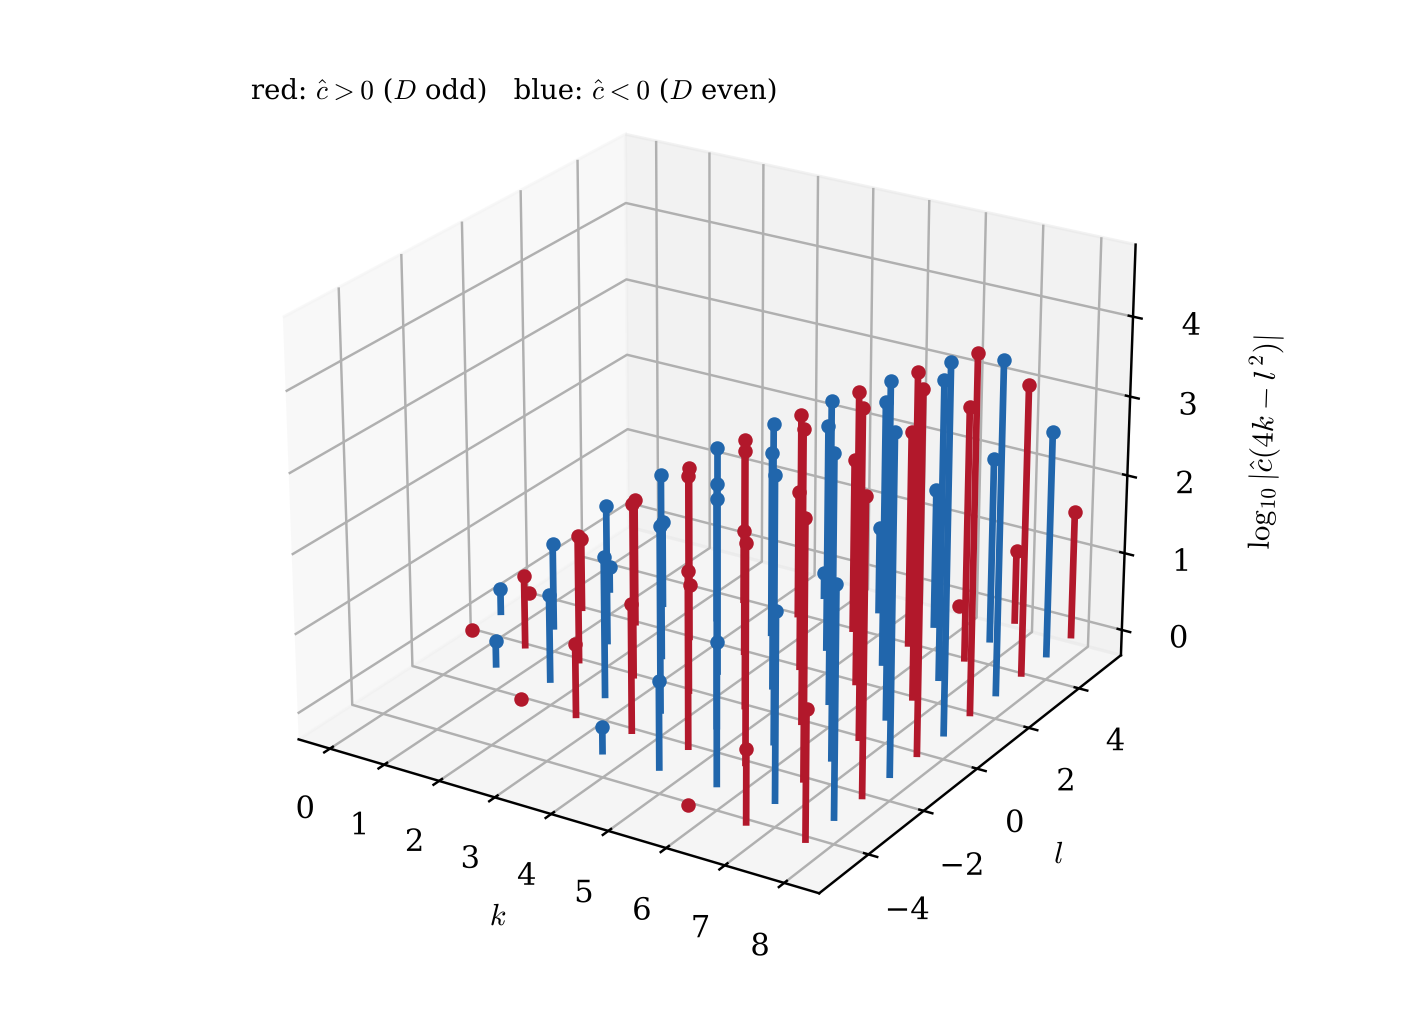
\includegraphics[width=0.78\textwidth]{fig_coefficients.png}
\caption{The coefficients $\cc(4k-l^2)$ of $\phi_{-2,1}$ for $k\le 8$, on a logarithmic scale. The sign is $(-1)^{D+1}$, and $|\cc|$ depends only on $D=4k-l^2$.}\label{fig:coeff}
\end{figure}

\begin{lemma}\label{lem:mono}
The sequence $a(n)$ is nondecreasing, and $a(n)-a(n-1)\ge\binom{n+4}{4}$ for $n\ge1$; also $a(n)\ge\binom{n+5}5$. For $D\ge3$ with $D\equiv0,3\pmod4$ put $k=\lfloor (D+1)/4\rfloor$ and $G(D)=|\cc(D)|-|\cc(D-4)|$. Then
\begin{equation}\label{eq:G}
G(D)\ge \begin{cases} a(k)-a(k-1), & D=4k-1,\\ 2\bigl(a(k)-a(k-1)\bigr), & D=4k.\end{cases}
\end{equation}
In particular $|\cc(D)|$ is strictly increasing on each of the classes $D\equiv 3$ and $D\equiv0\pmod 4$, $D\ge-1$. Moreover, for every $E\ge-1$,
\begin{equation}\label{eq:upper}
|\cc(E)|\le\bigl(\sqrt{E+1}+1\bigr)\,a\bigl(\lfloor (E+1)/4\rfloor\bigr).
\end{equation}
\end{lemma}

\begin{proof}
The series $(1-q)P(q)=(1-q)^{-5}\prod_{m\ge2}(1-q^m)^{-6}$ has nonnegative coefficients, and since the second factor has constant term $1$, its coefficient of $q^n$ is at least the coefficient $\binom{n+4}{4}$ of $(1-q)^{-5}$; hence $a(n)-a(n-1)\ge\binom{n+4}4>0$ for $n\ge1$. In the same way $P(q)=(1-q)^{-6}\prod_{m\ge2}(1-q^m)^{-6}$ gives $a(n)\ge\binom{n+5}5$. For $D=4k-1$, Lemma~\ref{lem:theta} gives
\[
G(D)=\sum_{m^2\le k}\bigl(a(k-m^2)-a(k-1-m^2)\bigr),
\]
a sum of nonnegative terms whose term $m=0$ is $a(k)-a(k-1)$. For $D=4k$ the same computation with $t(t+1)$ in place of $m^2$ and the factor $2$ gives the second case. In \eqref{eq:theta} the integers $j$ of fixed parity with $j^2\le E+1$ lie in an interval of length $2\sqrt{E+1}$ with spacing $2$, so there are at most $\sqrt{E+1}+1$ of them, and each argument of $a$ is at most $\lfloor(E+1)/4\rfloor$; since $a$ is nondecreasing, \eqref{eq:upper} follows.
\end{proof}

Two arithmetic facts link the charges with these coefficients.

\begin{lemma}\label{lem:arith}
Let $Q,P$ lie in an even lattice with integral bilinear form, and let $\ell_1,\ell_2$ and $\Delta$ be as in Section~\ref{sec:intro}. Then $\Delta\equiv Q\cdot P\pmod 2$, $\Delta\equiv0,3\pmod4$, and $\ell_1^2\mid\Delta$ and $\ell_2^2\mid\Delta$. If $\gcd(\ell_1,\ell_2)=1$, then $s^2\mid\Delta$ for every $s\mid\ell_1\ell_2$.
\end{lemma}

\begin{proof}
$Q^2$ and $P^2$ are even, so $Q^2P^2\equiv0\pmod4$ and $\Delta\equiv-(Q\cdot P)^2$, which is $\equiv Q\cdot P\pmod2$ and $\equiv0$ or $3\pmod4$ because a square is $0$ or $1$ modulo $4$. Writing $\Delta=4\cdot\frac{Q^2}2\cdot\frac{P^2}2-(Q\cdot P)^2$ shows $\ell_2^2\mid\Delta$. Let $L$ be the Gram matrix in a basis of the lattice, so that $Q\cdot P=Q^{\mathsf T}LP$. By Lagrange's identity (Appendix~\ref{app:standard}) applied to the vectors $Q,P,LQ,LP$,
\[
\Delta=(Q\cdot LQ)(P\cdot LP)-(Q\cdot LP)(P\cdot LQ)=\sum_{i<j}(Q\wedge P)_{ij}\,(LQ\wedge LP)_{ij},
\]
where the dot is now the Euclidean product of coordinate vectors. The vector $LQ\wedge LP=(\Lambda^2L)(Q\wedge P)$ has entries that are integral combinations of the entries of $Q\wedge P$. Both factors are divisible by $\ell_1$, so $\ell_1^2\mid\Delta$. If $\gcd(\ell_1,\ell_2)=1$ then $(\ell_1\ell_2)^2\mid\Delta$, and every divisor $s$ of $\ell_1\ell_2$ has $s^2\mid\Delta$.
\end{proof}

\section{Partitions into six colours}\label{sec:a}

The proof needs $a(n)$ bounded above at about half the argument and below at the full argument, with explicit constants. Figure~\ref{fig:abounds} shows the bounds of this section against the true values.

\begin{lemma}\label{lem:aupper}
For every $n\ge1$,
\[
a(n)\le 1.0001\,\frac{e^{2\pi\sqrt n}}{8n^{3/2}},\qquad\text{and}\qquad a(n)\le e^{2\pi\sqrt n}\quad(n\ge0).
\]
\end{lemma}

\begin{proof}
For $t>0$ the transformation $\eta(i/t)=\sqrt t\,\eta(it)$ \cite[Thm.~3.1]{Apo90} gives
\[
P(e^{-2\pi t})=e^{-\pi t/2}\eta(it)^{-6}=t^3e^{\pi/(2t)-\pi t/2}\prod_{m\ge1}\bigl(1-e^{-2\pi m/t}\bigr)^{-6}.
\]
Indeed $\eta(it)^{-6}=e^{\pi t/2}P(e^{-2\pi t})$ by the definition of $\eta$, and $\eta(it)^{-6}=t^3\eta(i/t)^{-6}=t^3e^{\pi/(2t)}\prod_m(1-e^{-2\pi m/t})^{-6}$. Since the coefficients of $P$ are nonnegative, $a(n)e^{-2\pi nt}\le P(e^{-2\pi t})$. Take $t=1/(2\sqrt n)$: then $2\pi nt=\pi/(2t)=\pi\sqrt n$, $t^3=1/(8n^{3/2})$ and $e^{-\pi t/2}<1$. With $x=e^{-2\pi/t}=e^{-4\pi\sqrt n}\le e^{-4\pi}<3.5\cdot10^{-6}$,
\[
-\log\prod_{m\ge1}(1-x^m)=\sum_{m\ge1}\sum_{r\ge1}\frac{x^{mr}}{r}\le\sum_{m\ge1}\frac{x^m}{1-x^m}\le\frac{x}{(1-x)^2},
\]
so the product raised to the power $-6$ is at most $\exp\bigl(6x/(1-x)^2\bigr)<1.0001$. The second bound is $a(0)=1$ for $n=0$; for $n\ge1$, $\frac{1.0001}{8n^{3/2}}<1$. Appendix~\ref{app:standard} gives a proof of the second bound that does not use the transformation of $\eta$.
\end{proof}

\begin{lemma}\label{lem:alower}
Let $b(n)$ be the coefficients of $\exp\bigl(6q/(1-q)\bigr)$, that is,
\[
b(0)=1,\qquad b(n)=\sum_{j=1}^{n}\frac{6^j}{j!}\binom{n-1}{j-1}\quad(n\ge1).
\]
Then $a(n)\ge b(n)$ for all $n\ge0$, and $b(n)\ge e^{2\sqrt{6n}-6}/n$ for $n\ge50$.
\end{lemma}

\begin{proof}
Logarithmic differentiation of $P(q)=\exp\bigl(6\sum_{m\ge1}\sum_{r\ge1}q^{mr}/r\bigr)$ and of $\exp(6\sum_{i\ge1}q^i)$ gives
\[
n\,a(n)=6\sum_{i=1}^n\sigma(i)\,a(n-i),\qquad n\,b(n)=6\sum_{i=1}^n i\,b(n-i),
\]
where $\sigma(i)$ is the sum of the divisors of $i$; indeed $q\frac d{dq}\sum_{m,r}q^{mr}/r=\sum_{m,r}mq^{mr}=\sum_i\sigma(i)q^i$. Since $\sigma(i)\ge i$ and $a(0)=b(0)=1$, induction on $n$ gives $a(n)\ge b(n)\ge0$. The closed form follows from $\exp(6u)=\sum_j6^ju^j/j!$ with $u=q/(1-q)$ and $u^j=\sum_{n\ge j}\binom{n-1}{j-1}q^n$.

For the lower bound let $x=\sqrt{6n}$, $j=\lfloor x\rfloor$ and $\theta=x-j\in[0,1)$; note $1\le j\le n$. Keeping one term,
\[
b(n)\ge\frac{6^j}{j!}\binom{n-1}{j-1}=\frac{6^j}{j!}\cdot\frac jn\binom nj=\frac{(6n)^j\,j}{n\,(j!)^2}\prod_{i<j}\Bigl(1-\frac in\Bigr).
\]
Robbins' form of Stirling's formula \cite{Rob55} is $j!\le\sqrt{2\pi j}\,(j/e)^je^{1/(12j)}$. It gives $(j!)^2\le 2\pi j\,(j/e)^{2j}e^{1/(6j)}$, and so
\[
\frac{(6n)^j j}{(j!)^2}\ge\frac{e^{2j}}{2\pi}\Bigl(\frac xj\Bigr)^{2j}e^{-1/(6j)}\ge \frac{e^{2x}}{2\pi}\,e^{-2\theta^2/x-1/(6j)},
\]
because $(x/j)^{2j}=(1-\theta/x)^{-2j}\ge e^{2j\theta/x}$ and therefore $e^{2j}(x/j)^{2j}\ge e^{2x-2\theta+2(x-\theta)\theta/x}=e^{2x-2\theta^2/x}\ge e^{2x-2/x}$. For $0\le y\le\frac12$ we have $\log(1-y)\ge-y-y^2$ (Appendix~\ref{app:standard}), and $i/n<j/n\le\sqrt{6/n}<\frac12$. Since $j(j-1)\le x(x-1)=6n-x$ and $\sum_{i<j}i^2\le j^3/3\le x^3/3=2nx$,
\[
\log\prod_{i<j}\Bigl(1-\frac in\Bigr)\ge-\frac{j(j-1)}{2n}-\frac{1}{n^2}\sum_{i<j}i^2\ge-3+\frac{x}{2n}-\frac{2x}{n}=-3-\frac{3x}{2n}.
\]
Altogether $n\,b(n)\,e^{-2x}\ge\exp\bigl(-\log(2\pi)-3-2/x-3x/(2n)-1/(6j)\bigr)$. The three last terms decrease in $n$; at $n=50$ they are $0.116$, $0.520$ and $0.010$, and $\log(2\pi)+3=4.838$. The exponent is therefore at least $-5.49>-6$.
\end{proof}

\begin{lemma}\label{lem:diff}
For $n\ge1$, $a(n)-a(n-1)\ge \dfrac{5}{n+5}\,a(n)$.
\end{lemma}

\begin{proof}
Let $w(i)\ge0$ be the coefficients of $\prod_{m\ge2}(1-q^m)^{-6}$. Then $P=(1-q)^{-6}\sum w(i)q^i$ and $(1-q)P=(1-q)^{-5}\sum w(i)q^i$, so
\[
a(n)=\sum_{i=0}^nw(n-i)\binom{i+5}{5},\qquad a(n)-a(n-1)=\sum_{i=0}^nw(n-i)\binom{i+4}{4}.
\]
Since $\binom{i+4}4=\frac5{i+5}\binom{i+5}5\ge\frac5{n+5}\binom{i+5}5$ for $i\le n$, the claim follows.
\end{proof}

Combining \eqref{eq:G} with Lemmas~\ref{lem:alower} and~\ref{lem:diff}: for $D\ge3$, $D\equiv0,3\pmod4$ and $k=\lfloor(D+1)/4\rfloor\ge50$,
\begin{equation}\label{eq:Glower}
G(D)\ge e^{\Lambda(k)},\qquad \Lambda(k)=2\sqrt{6k}-6-\log k+\log\frac{5}{k+5}.
\end{equation}

\begin{figure}[ht]
\centering
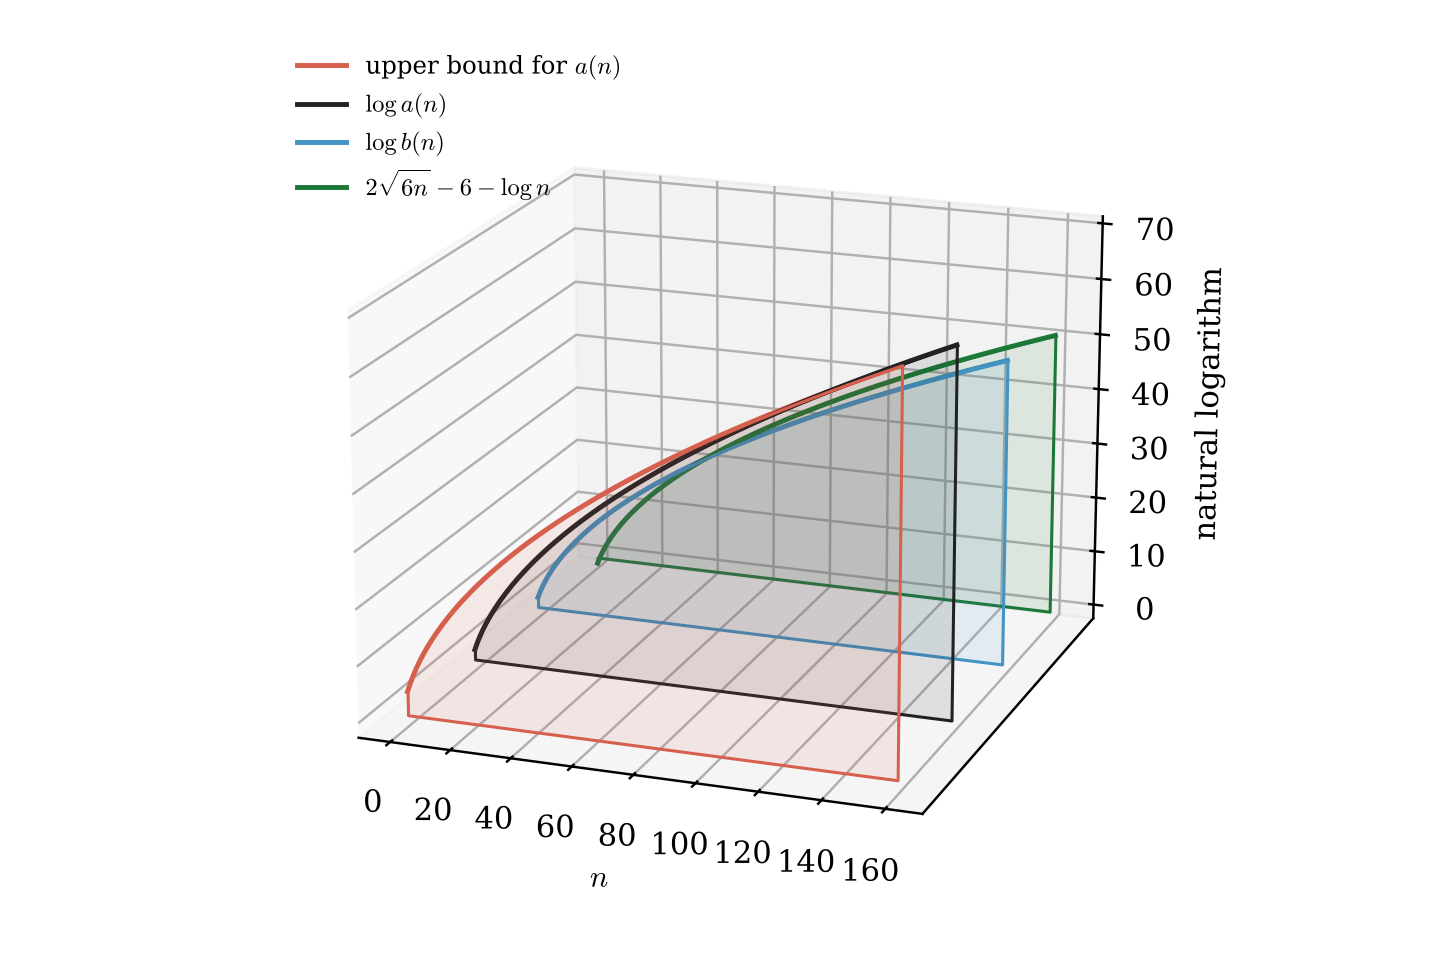
\includegraphics[width=0.8\textwidth]{fig_abounds.png}
\caption{From front to back: the upper bound of Lemma~\ref{lem:aupper}, the true values $\log a(n)$, the comparison series $\log b(n)$ of Lemma~\ref{lem:alower}, and its explicit lower bound $2\sqrt{6n}-6-\log n$, for $n\le160$. The lower bound grows like $2\sqrt6\sqrt n$ instead of $2\pi\sqrt n$; Proposition~\ref{prop:key} needs only that it beats the upper bound taken at a quarter of the argument.}\label{fig:abounds}
\end{figure}

\section{The key inequality}\label{sec:key}

For $E\ge1$ put
\[
W(E)=\sum_{\substack{s\ge2\\ s^2\mid E}}s^2\,\bigl|\cc(E/s^2)\bigr|,\qquad W^*(D)=\max_{1\le E\le D}W(E),
\]
and $W(E)=0$ for $E\le0$. So $W(E)$ bounds every divisor sum $\sum_{s\ge2}w(s)\cc(E/s^2)$ with $|w(s)|\le s^2$.

\begin{proposition}\label{prop:key}
For every $D\ge3$ with $D\equiv0,3\pmod4$,
\begin{align}
&G(D)>2\,W^*(D),\label{eq:keya}\\
&G(D)>W^*(D)+\tfrac1{16}(D+4)(D+8).\label{eq:keyb}
\end{align}
\end{proposition}

\begin{proof}
\emph{The range $D\ge359$.} Here $k=\lfloor(D+1)/4\rfloor\ge\Kzero$ and $D\le4k$. Let $1\le E\le D$. Every term of $W(E)$ has $E/s^2\ge1$, and by \eqref{eq:upper} it is at most $s^2(\sqrt{E/s^2+1}+1)\,a(\lfloor(E/s^2+1)/4\rfloor)$, which increases with $E$. The term $s=2$ is therefore at most
\[
4\bigl(\sqrt{k+1}+1\bigr)a\bigl(\lfloor(k+1)/4\rfloor\bigr)\le S_2(k):=1.0001\cdot\frac{4(\sqrt{k+1}+1)}{(k+1)^{3/2}}\,e^{\pi\sqrt{k+1}},
\]
by Lemma~\ref{lem:aupper} and because $e^{2\pi\sqrt y}y^{-3/2}$ increases for $y\ge1$ (its logarithmic derivative is $\pi/\sqrt y-3/(2y)>0$), evaluated at $y=(k+1)/4\ge\lfloor(k+1)/4\rfloor$. For $s\ge3$ the factors $\sqrt{E/s^2+1}+1$ and $a(\cdot)$ are largest at $s=3$, and $\sum_{3\le s\le\sqrt E}s^2\le\lfloor\sqrt E\rfloor^3\le E^{3/2}\le(4k)^{3/2}$, since $\sum_{s=1}^Ns^2=\frac16N(N+1)(2N+1)\le N^3$. With the second bound of Lemma~\ref{lem:aupper},
\[
\sum_{s\ge3}\le S_3(k):=(4k)^{3/2}\Bigl(\sqrt{4k/9+1}+1\Bigr)e^{\frac{2\pi}3\sqrt{k+9/4}}.
\]
So $W^*(D)\le S_2(k)+S_3(k)$, and $\tfrac1{16}(D+4)(D+8)\le(k+1)(k+2)$. Put $S_4(k)=2(k+1)(k+2)$. If
\begin{equation}\label{eq:hi}
h_i(k):=\Lambda(k)-\log4-\log S_i(k)>0\qquad(i=2,3,4),
\end{equation}
then by \eqref{eq:Glower} $G(D)>4\max(S_2,S_3)\ge2(S_2+S_3)\ge2W^*(D)$, which is \eqref{eq:keya}, and $G(D)>4S_4(k)$, so that $G(D)-W^*(D)>\tfrac12G(D)>2S_4(k)>\tfrac1{16}(D+4)(D+8)$, which is \eqref{eq:keyb}.

At $k=\Kzero$,
\[
\Lambda(\Kzero)=33.03,\qquad \log4+\log S_2=28.33,\qquad \log4+\log S_3=32.33,\qquad\log4+\log S_4=11.11 .
\]
For the derivatives, $\Lambda'(k)=\sqrt6/\sqrt k-1/k-1/(k+5)\ge\sqrt6/\sqrt k-2/k$. Differentiating the logarithms and discarding the negative terms,
\[
(\log S_2)'\le\frac{\pi}{2\sqrt k}+\frac1{2k},\qquad(\log S_3)'\le\frac{\pi}{3\sqrt k}+\frac{2}{k},\qquad (\log S_4)'\le\frac2k .
\]
For $S_2$ the derivative of $\log(\sqrt{k+1}+1)$ is $\bigl(2(k+1+\sqrt{k+1})\bigr)^{-1}<\frac1{2k}$. For $S_3$ the derivative of $\frac32\log(4k)$ is $\frac3{2k}$, and with $y=4k/9+1$ the derivative of $\log(\sqrt y+1)$ is $\frac{2}{9(y+\sqrt y)}<\frac2{9y}<\frac1{2k}$. Hence
\[
h_2'\ge\frac{0.878}{\sqrt k}-\frac{2.5}k,\qquad h_3'\ge\frac{1.402}{\sqrt k}-\frac{4}{k},\qquad h_4'\ge\frac{2.449}{\sqrt k}-\frac4k,
\]
all positive for $k\ge9$. So \eqref{eq:hi} holds for every $k\ge\Kzero$.\footnote{Lemma~\ref{lem:alower} requires $k\ge50$, which holds. The inequalities \eqref{eq:hi} already hold for $k\ge84$; the choice $\Kzero$ leaves a margin of $0.7$ in the tightest one, see Figure~\ref{fig:exp}.}

\emph{The range $3\le D\le358$.} Here every quantity in \eqref{eq:keya} and \eqref{eq:keyb} is an integer determined by $a(0),\dots,a(89)$ through \eqref{eq:theta}. Appendix~\ref{app:finite} describes the computation, which compares integers only. Both inequalities hold; the largest value of $2W^*(D)/G(D)$ is $64/152=0.421$, at $D=12$, and the largest value of $\bigl(W^*(D)+\frac1{16}(D+4)(D+8)\bigr)/G(D)$ is $\frac{77}{112}=0.6875$, at $D=3$, where $W^*(3)=0$ and $G(3)=8-1=7$. Figure~\ref{fig:margins} shows both ratios.
\end{proof}

\begin{figure}[ht]
\centering
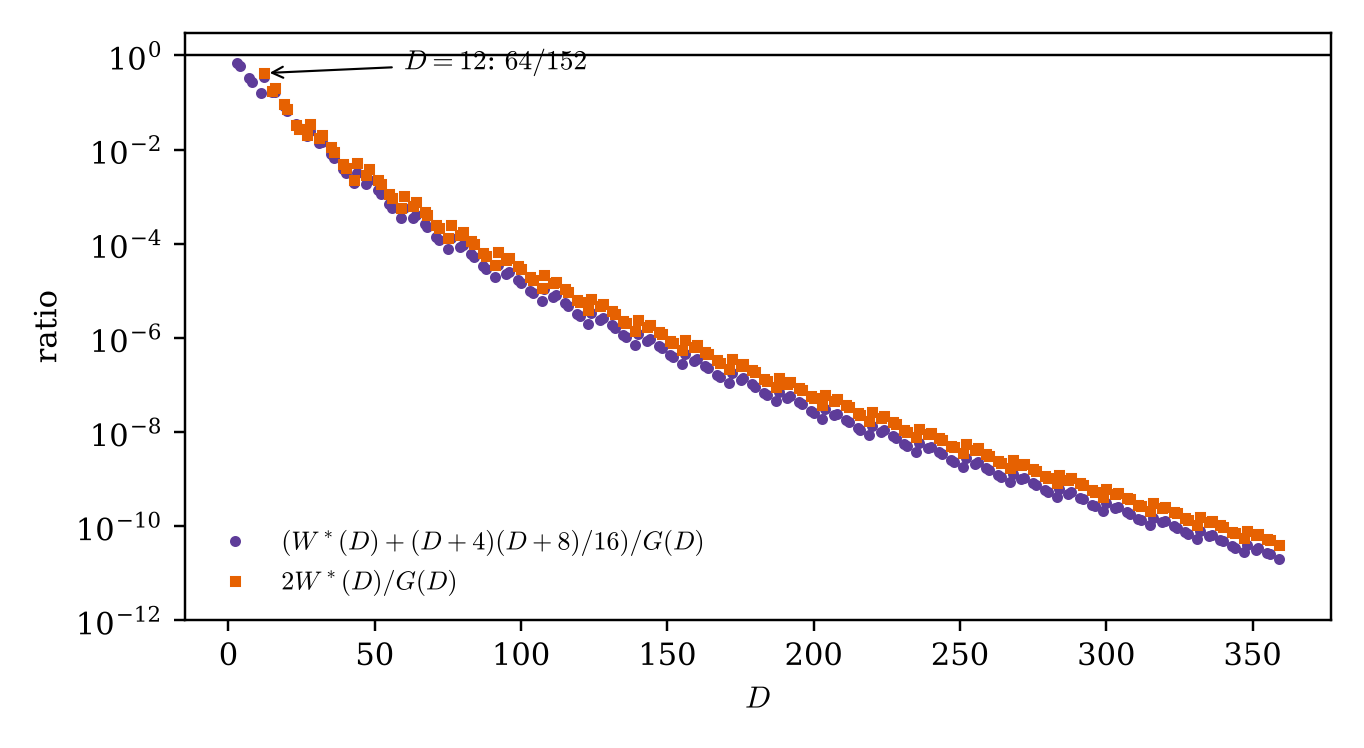
\includegraphics[width=0.78\textwidth]{fig_margins.png}
\caption{The two ratios of Proposition~\ref{prop:key} for $3\le D\le 359$. Both stay below $1$, with the largest values at the smallest discriminants, and fall off like $e^{-c\sqrt D}$.}\label{fig:margins}
\end{figure}

\begin{figure}[ht]
\centering
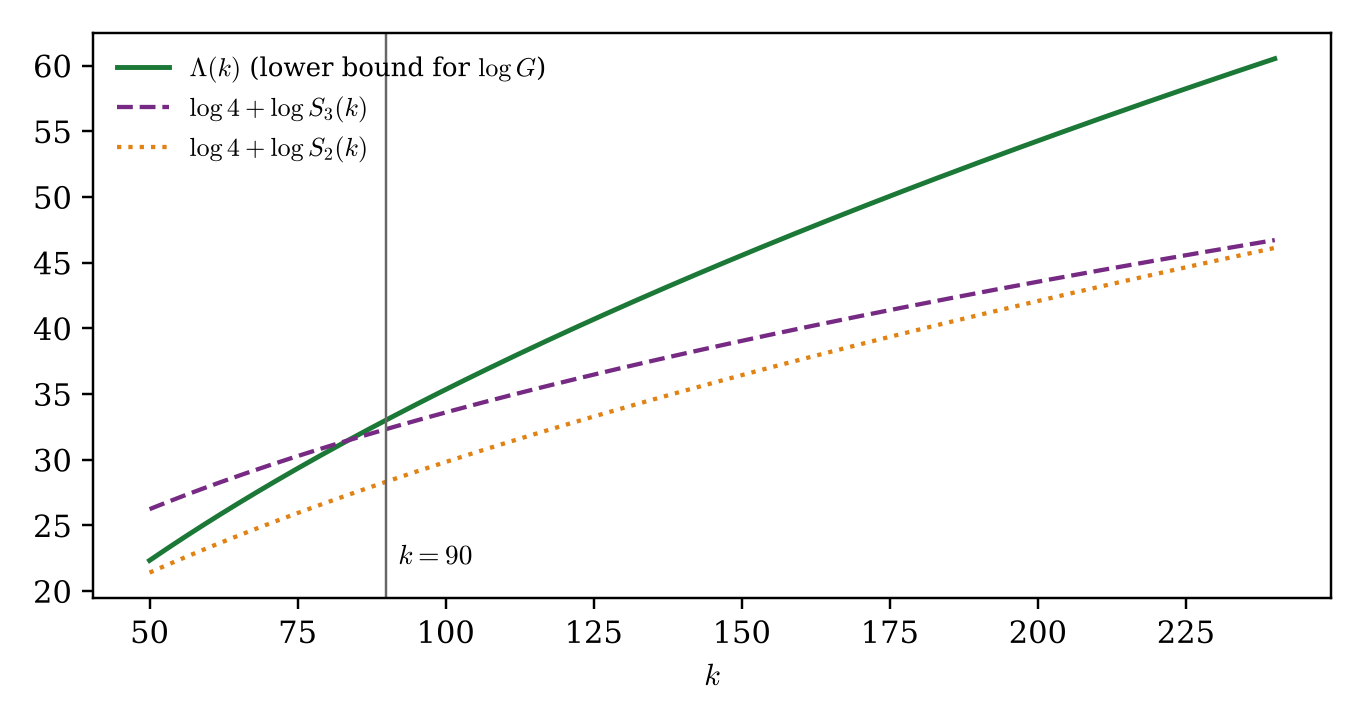
\includegraphics[width=0.78\textwidth]{fig_exponents.png}
\caption{The lower bound $\Lambda(k)$ for $\log G(D)$ against the upper bounds $\log4+\log S_i(k)$ for the divisor sums. The analytic argument applies from $k=\Kzero$ on.}\label{fig:exp}
\end{figure}

The inequality is used in the following form.

\begin{corollary}\label{cor:principle}
Let $D\ge3$ with $D\equiv0,3\pmod4$, and let $w(s)$, for the integers $s\ge1$ with $s^2\mid D$, be real numbers with $w(1)=1$ and $|w(s)|\le s^2$. Then
\[
(-1)^{D+1}\sum_{s^2\mid D}w(s)\,\cc(D/s^2)\ \ge\ |\cc(D)|-W(D)\ >\ \tfrac12|\cc(D)|.
\]
\end{corollary}

\begin{proof}
The term $s=1$ is $(-1)^{D+1}\cc(D)=|\cc(D)|$ by Lemma~\ref{lem:theta}, and the others add up to at most $W(D)$ in absolute value. By \eqref{eq:keya}, $W(D)\le W^*(D)<\frac12G(D)\le\frac12|\cc(D)|$.
\end{proof}

\section{Four-dimensional dyons}\label{sec:4d}

\begin{proof}[Proof of Theorem~\ref{thm:A}]
By Lemma~\ref{lem:arith}, $\Delta\equiv0,3\pmod4$, so $\Delta>0$ forces $\Delta\ge3$; $s^2\mid\Delta$ for every $s\mid\ell_1\ell_2$; and $(-1)^{Q\cdot P+1}=(-1)^{\Delta+1}$. Hence
\[
d(Q,P)=(-1)^{\Delta+1}\sum_{s^2\mid\Delta}w(s)\,\cc(\Delta/s^2),\qquad w(s)=\begin{cases}s,&s\mid\ell_1\ell_2,\\0,&\text{otherwise},\end{cases}
\]
and $0\le w(s)\le s\le s^2$, $w(1)=1$. Corollary~\ref{cor:principle} gives $d(Q,P)>\frac12|\cc(\Delta)|$.
\end{proof}

The proof uses neither the parity of $s$ nor the sign of $w(s)$; only $|w(s)|\le s^2$ enters, and the weights of \eqref{eq:d4} are smaller by a factor $s$. By Lemma~\ref{lem:invariants} the index depends on the charges only through $\Delta$, $\ell_1\ell_2$ and the parity of $Q\cdot P$, which is the parity of $\Delta$.

Table~\ref{tab:ex4d} lists the index for small charges in Sen's normal form of Section~\ref{ssec:charges}, realised as $Q=\ell_1(e_1+nf_1)$, $P=e_2+mf_2+pf_1$ in two hyperbolic planes, so that $\frac12Q^2=\ell_1^2n$, $\frac12P^2=m$, $Q\cdot P=\ell_1p$, and $Q_0\wedge P_0$ is primitive because its $(e_1,e_2)$ entry is $1$. The terms of \eqref{eq:d4} are listed with their signs. A negative term occurs exactly when $s$ is even and $\Delta/s^2$ has the parity opposite to $\Delta$, as for $\Delta=12,28,44$ with $s=2$ and $\Delta=48$ with $s=4$; in every case it is a tiny fraction of the leading term. Figure~\ref{fig:index4d} shows the growth of the index.\footnote{The rows with $\ell_1=2,3$ have the same $\Delta$ and $\ell_1\ell_2$ as rows with $\ell_1=1$ and the same index, as Lemma~\ref{lem:invariants} and \eqref{eq:d4} require.}

\begin{table}[ht]\centering\footnotesize
\caption{The index $d(Q,P)$ of \eqref{eq:d4} for small charges with $\gcd(\ell_1,\ell_2)=1$. The column ``terms'' lists $(-1)^{Q\cdot P+1}s\,\cc(\Delta/s^2)$ for the divisors $s=1<s_2<\dots$ of $\ell_1\ell_2$.}\label{tab:ex4d}
\begin{tabular}{@{}rrrrrrlr@{}}\toprule
$\frac12Q^2$ & $\frac12P^2$ & $Q\cdot P$ & $\ell_1$ & $\ell_2$ & $\Delta$ & terms & $d(Q,P)$\\\midrule
1 & 1 & 0 & 1 & 1 & 4 & $12$ & 12\\
1 & 1 & 1 & 1 & 1 & 3 & $8$ & 8\\
2 & 1 & 1 & 1 & 1 & 7 & $39$ & 39\\
2 & 2 & 0 & 1 & 2 & 16 & $684$ $+24$ & 708\\
2 & 2 & 1 & 1 & 1 & 15 & $513$ & 513\\
2 & 2 & 2 & 1 & 2 & 12 & $208$ $-16$ & 192\\
3 & 3 & 3 & 1 & 3 & 27 & $11552$ $+24$ & 11576\\
2 & 4 & 2 & 1 & 2 & 28 & $14592$ $-78$ & 14514\\
4 & 4 & 4 & 1 & 4 & 48 & $928720$ $+416$ $-32$ & 929104\\
4 & 4 & 0 & 1 & 4 & 64 & $15740076$ $+1368$ $+48$ & 15741492\\
6 & 6 & 6 & 1 & 6 & 108 & $10744220992$ $-23104$ $+624$ $-48$ & 10744198464\\
4 & 1 & 2 & 2 & 1 & 12 & $208$ $-16$ & 192\\
9 & 1 & 3 & 3 & 1 & 27 & $11552$ $+24$ & 11576\\
4 & 3 & 2 & 2 & 1 & 44 & $431984$ $-304$ & 431680\\
\bottomrule\end{tabular}\end{table}

\begin{figure}[ht]
\centering
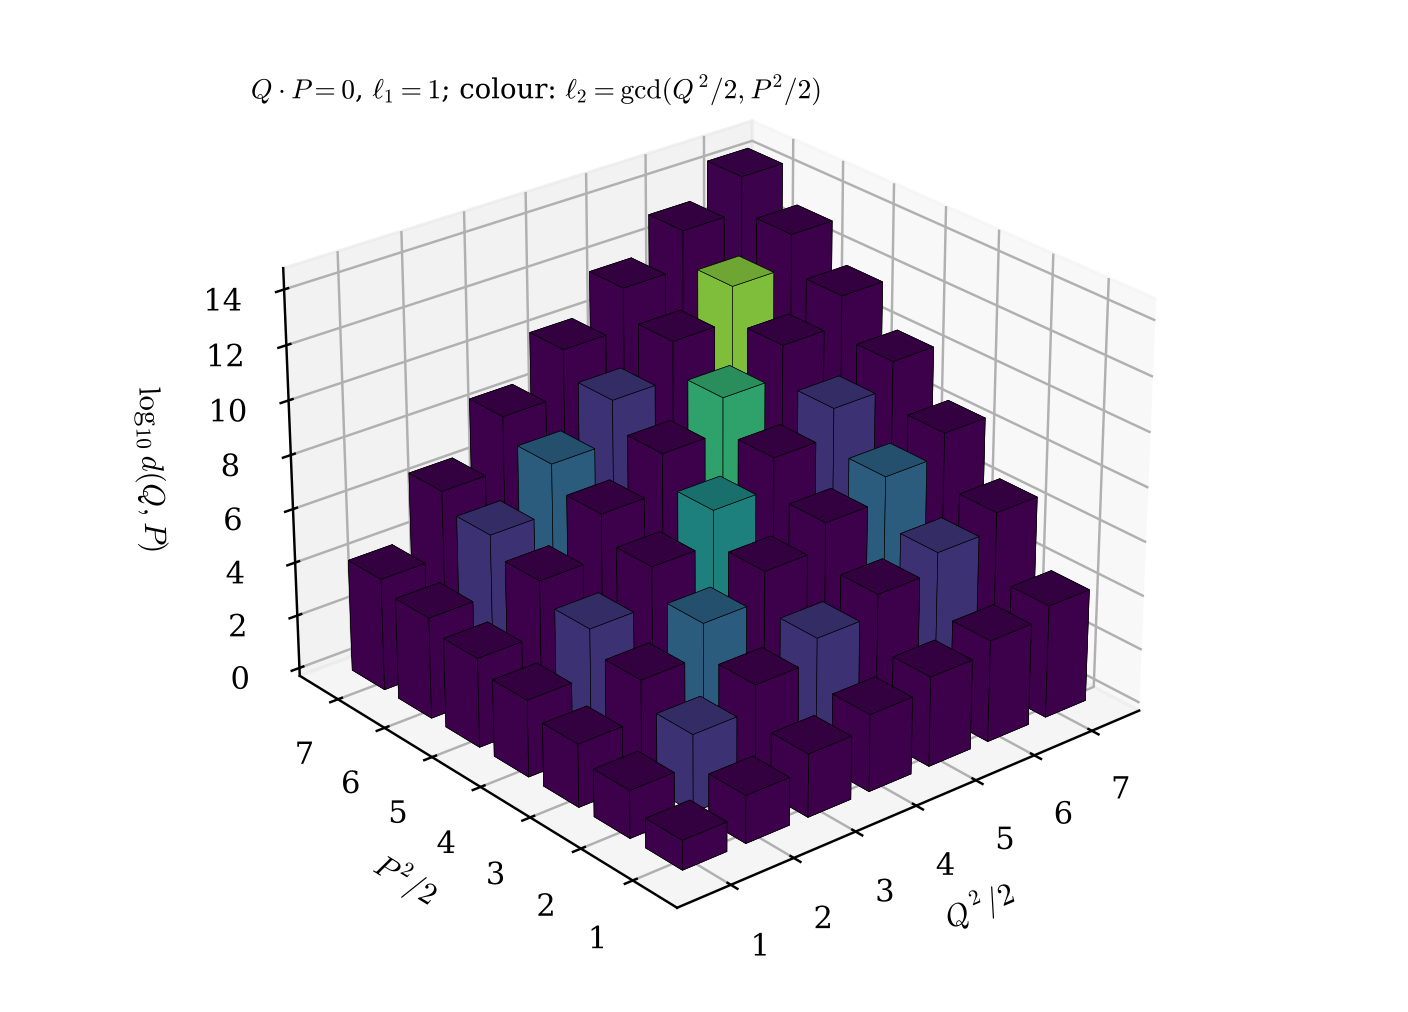
\includegraphics[width=0.74\textwidth]{fig_index4d.png}
\caption{The index $d(Q,P)$ for $Q\cdot P=0$, $\ell_1=1$ and $1\le\frac12Q^2,\frac12P^2\le7$, on a logarithmic scale; the colour shows $\ell_2$. The diagonal carries the largest $\ell_2$ and hence the most divisor terms, without visible effect on the size.}\label{fig:index4d}
\end{figure}

\section{Five-dimensional black holes}\label{sec:5d}

Fix $Q_1,Q_5,n\ge1$ with $\gcd(Q_1,Q_5)=1$, put $M=Q_1Q_5n$ and $g=\gcd(n,Q_1Q_5)$, and for $l\in\ZZ$ write $D(l)=4M-l^2$ and
\[
\varepsilon(l)=(-1)^{l+1}F(l),
\]
with $F$ as in \eqref{eq:F}. If $s\mid g$ then $s\mid n$ and $s\mid Q_1Q_5$, so $s^2\mid M$; if moreover $s\mid l$, then $s^2\mid D(l)$. Since $F(-l)=F(l)$, $\varepsilon$ is an even function of $l$. Note that $D(l)\equiv l\pmod 2$ and $D(l)\equiv0,3\pmod4$.

\begin{lemma}\label{lem:eps}
\begin{enumerate}
\item If $D(l)\ge3$, then $\varepsilon(l)\ge|\cc(D(l))|-W(D(l))>\frac12|\cc(D(l))|$.
\item If $D(l)=0$, then $\varepsilon(l)=2\sigma\bigl(\gcd(g,l)\bigr)$; if $D(l)=-1$, then $\varepsilon(l)=1$.
\item If $D(l)<-1$, then $\varepsilon(l)=(-1)^{l+1}s_0$ when $D(l)=-s_0^2$ with $s_0\ge2$ and $s_0\mid\gcd(g,l)$, and $\varepsilon(l)=0$ otherwise. In the first case $l\equiv s_0\pmod 2$, so $\varepsilon(l)=s_0>0$ for odd $l$ and $\varepsilon(l)=-s_0<0$ for even $l$.
\end{enumerate}
\end{lemma}

\begin{proof}
Since $(-1)^{l+1}=(-1)^{D(l)+1}$, (1) is Corollary~\ref{cor:principle} with $w(s)=s$ for $s\mid\gcd(g,l)$ and $w(s)=0$ otherwise. If $D(l)=0$ then $l$ is even and every $s\mid\gcd(g,l)$ contributes $s\,\cc(0)=-2s$, so $\varepsilon(l)=2\sigma(\gcd(g,l))$. If $D(l)=-1$, only $s=1$ has $s^2\mid D(l)$, $l$ is odd and $\varepsilon(l)=\cc(-1)=1$. If $D(l)<-1$, a term $s$ of \eqref{eq:F} is nonzero only if $D(l)/s^2\ge-1$, that is $s^2\ge-D(l)$; since $s^2$ divides $D(l)$, this means $s^2=-D(l)$. So there is at most one nonzero term, $s=s_0=\sqrt{-D(l)}$, present when $s_0$ is an integer dividing $\gcd(g,l)$, and it equals $s_0\cc(-1)=s_0$. Finally $l\equiv D(l)=-s_0^2\equiv s_0\pmod 2$.
\end{proof}

The values in (3) are the polar terms. They are nonzero only when $g>1$, and they are small, but they enter \eqref{eq:d5} and \eqref{eq:drot} with fixed signs and have to be controlled. The next lemma ties their size to the discriminant of a nearby $l$.

\begin{lemma}\label{lem:polar}
Let $0\le l_1<l_2$ with $D(l_1)\ge3$, and suppose $D(l_2)=-s_0^2$ with $s_0\ge2$ and $s_0\mid\gcd(g,l_2)$. Put $t=l_2-l_1$ and $\lambda=l_2/s_0$. Then $\lambda$ is odd, $\lambda\ge3$, and
\[
D(l_1)+t^2=s_0\,u,\qquad u=2t\lambda-s_0,
\]
where $u$ is a positive integer with $u\equiv s_0\pmod 2$. In particular $s_0\le D(l_1)+t^2$, and $s_0\le\frac12\bigl(D(l_1)+t^2\bigr)$ when $s_0$ is even.
\end{lemma}

\begin{proof}
As noted above, $s_0\mid g$ gives $s_0^2\mid M$; put $\mu=M/s_0^2\ge1$. Dividing $4M-l_2^2=-s_0^2$ by $s_0^2$ gives $\lambda^2=4\mu+1\ge5$, so $\lambda$ is odd and at least $3$. Next,
\[
D(l_1)=4M-(l_2-t)^2=\bigl(4M-l_2^2\bigr)+2tl_2-t^2=-s_0^2+2ts_0\lambda-t^2,
\]
which is the identity. Its left side is positive, so $u\ge1$, and $u=2t\lambda-s_0\equiv s_0\pmod 2$. If $s_0$ is even then $u\ge2$.
\end{proof}

For example $Q_1=11$, $Q_5=1$, $n=22$ give $M=242$ and $g=11$; at $l=33$, $D(33)=968-1089=-121$ and $\varepsilon(33)=11$. With $l_1=31$ we have $D(31)=7$, $t=2$, $\lambda=3$ and $7+4=11\cdot1$. Lemma~\ref{lem:polar} is sharp here. Figure~\ref{fig:pairing} shows this charge.

Since $(-1)^{J+1}(-1)^r=(-1)^{(J-r)+1}$, the definition \eqref{eq:d5} becomes
\begin{equation}\label{eq:d5eps}
\dt(n,Q_1,Q_5,J)=\sum_{r=-2}^{2}\binom{4}{2-r}\varepsilon(J-r).
\end{equation}

\begin{proof}[Proof of Theorem~\ref{thm:B}]
Since $\dt$ is even in $J$, we may assume $J\ge0$. Put $D=D(J)$; then $D\ge3$, because $D>0$ and $D\equiv0,3\pmod4$. The term $r=0$ of \eqref{eq:d5eps} is $6\varepsilon(J)>3|\cc(D)|$ by Lemma~\ref{lem:eps}(1). The other terms have $l=J-r$ with $r\ne0$. If $D(l)\ge-1$ the term is nonnegative by Lemma~\ref{lem:eps}. If $D(l)<-1$ then $l^2>J^2$, so $|l|=J+t$ with $t\in\{1,2\}$; the term is negative only if $|l|$ is even and $D(l)=-s_0^2$ with $s_0$ even, and then, by Lemma~\ref{lem:polar} with $l_1=J$ and $l_2=|l|$, it is at least $-\binom4{2-r}\cdot\frac12(D+4)$. For $J\ge1$ the values $|l|>J$ are $J+1$ and $J+2$, with coefficients $4$ and $1$; for $J=0$ the even ones are $l=\pm2$, with coefficients $1$ and $1$. In all cases
\[
\dt(n,Q_1,Q_5,J)>3|\cc(D)|-\tfrac52(D+4).
\]
For $D=3,4$ the right side is $24-17.5$ and $36-20$. For $D\ge7$ put $k=\lfloor(D+1)/4\rfloor\ge2$; then $D\le 4k$, and by Lemma~\ref{lem:theta} and Lemma~\ref{lem:mono}, $|\cc(D)|\ge a(k)\ge\binom{k+5}5\ge(k+5)(k+1)$, since $(k+4)(k+3)(k+2)\ge120$. So $3|\cc(D)|\ge3k^2+18k+15>10k+10\ge\frac52(D+4)$.
\end{proof}

In the index at fixed $J$ the terms no longer have the same sign, and the monotonicity of the coefficients has to absorb the difference.

\begin{lemma}\label{lem:pair}
Let $0\le l_1<l_2$ with $l_1\equiv l_2\pmod 2$ and $D(l_1)\ge3$.
\begin{enumerate}
\item If $D(l_2)\ge-1$, then $\varepsilon(l_1)>\varepsilon(l_2)$.
\item If $D(l_2)<-1$ and $l_2-l_1\le6$, then $\varepsilon(l_1)>\varepsilon(l_2)$.
\end{enumerate}
\end{lemma}

\begin{proof}
Put $D_1=D(l_1)$ and $D_2=D(l_2)$. Then $D_1-D_2=(l_2-l_1)(l_2+l_1)$ is a product of two even numbers, both at least $2$, so $D_2\le D_1-4$ and $D_2\equiv D_1\pmod 4$. By Lemma~\ref{lem:mono}, $|\cc(D_1)|-|\cc(D_2)|\ge G(D_1)$ whenever $D_2\ge-1$.

(1) If $D_2\ge3$, Lemma~\ref{lem:eps} and \eqref{eq:keya} give
\[
\varepsilon(l_1)-\varepsilon(l_2)\ge|\cc(D_1)|-|\cc(D_2)|-W(D_1)-W(D_2)\ge G(D_1)-2W^*(D_1)>0 .
\]
If $D_2=-1$, then $\varepsilon(l_2)=1=|\cc(-1)|$ and $\varepsilon(l_1)-\varepsilon(l_2)\ge G(D_1)-W^*(D_1)>0$.

If $D_2=0$, then $l_2^2=4M$ and $\varepsilon(l_2)=2\sigma(m)$ with $m=\gcd(g,l_2)\le l_2$. Since $l_1\le l_2-2$, $D_1\ge l_2^2-(l_2-2)^2=4l_2-4$, so $m\le l_2\le\frac14(D_1+4)$. With $|\cc(0)|=2$ and $\sigma(m)\le\frac12m(m+1)$ (Appendix~\ref{app:standard}),
\[
\varepsilon(l_1)-\varepsilon(l_2)\ge\bigl(|\cc(D_1)|-|\cc(0)|\bigr)-W(D_1)-2\bigl(\sigma(m)-1\bigr)\ge G(D_1)-W^*(D_1)-m(m+1),
\]
and $m(m+1)\le\frac1{16}(D_1+4)(D_1+8)$. The right side is positive by \eqref{eq:keyb}.

(2) By Lemma~\ref{lem:eps}(3) we may assume $\varepsilon(l_2)>0$, since otherwise $\varepsilon(l_2)\le0<\varepsilon(l_1)$. Then $l_2$ is odd, $D(l_2)=-s_0^2$ with $s_0$ odd, $s_0\ge3$, and $\varepsilon(l_2)=s_0$. Also $l_1$ is odd, so $D_1$ is odd and $D_1\equiv3\pmod4$; and $t=l_2-l_1\in\{2,4,6\}$. Lemma~\ref{lem:polar} gives $s_0\le D_1+t^2\le D_1+36$.

Suppose $D_1\ge11$ and write $D_1=4k-1$ with $k\ge3$. For $k=3$, $\varepsilon(l_1)>\frac12|\cc(11)|=76>47$. For $k\ge4$, $\varepsilon(l_1)>\frac12|\cc(D_1)|\ge\frac12a(k)\ge\frac12\binom{k+5}5$; this is $63$ at $k=4$ and grows by $\frac12\binom{k+4}4\ge35$ with each step, while $D_1+36=4k+35$ is $51$ at $k=4$ and grows by $4$. In both cases $\varepsilon(l_1)>D_1+36\ge s_0$.

Suppose $D_1\in\{3,7\}$. By Lemma~\ref{lem:polar}, $s_0u=D_1+t^2$ and $s_0+u=2t\lambda$ with $\lambda$ odd and $\lambda\ge3$, so $s_0+u$ is $4\lambda$, $8\lambda$ or $12\lambda$ for $t=2,4,6$. The products $D_1+t^2$ are $7,19,39$ for $D_1=3$ and $11,23,43$ for $D_1=7$; their factorisations $s_0u$ have $s_0+u\in\{8\}$, $\{20\}$, $\{16,40\}$ and $\{12\}$, $\{24\}$, $\{44\}$. The only sums of the required form are $12=4\cdot3$ and $24=8\cdot3$, both for $D_1=7$, with $s_0=11$ and $s_0=23$. Then $\varepsilon(l_1)\ge|\cc(7)|-W(7)=39>23\ge s_0$, and for $D_1=3$ no polar value occurs.
\end{proof}

The case $D_2=0$ is the only place where a divisor sum enters with no small factor in front of it: all its terms carry the same sign as the leading term of $\varepsilon(l_2)$, and they are subtracted. This is the reason for the second inequality of Proposition~\ref{prop:key}.

\begin{proof}[Proof of Theorem~\ref{thm:C}]
By \eqref{eq:drot} and \eqref{eq:d5eps}, collecting the coefficient of each $\varepsilon(J-u)$,
\[
d(n,Q_1,Q_5,J)=\varepsilon(J-2)+4\varepsilon(J-1)+5\varepsilon(J)-5\varepsilon(J+2)-4\varepsilon(J+3)-\varepsilon(J+4),
\]
since the coefficients of $(\zeta^{1/2}-\zeta^{-1/2})^4(1-\zeta^{-2})$ are $1,-4,5,0,-5,4,-1$. Hence
\[
d(n,Q_1,Q_5,J)=\sum_{r=0}^{2}c_r\bigl(\varepsilon(|J-r|)-\varepsilon(J+2+r)\bigr),\qquad (c_0,c_1,c_2)=(5,4,1),
\]
using that $\varepsilon$ is even. Put $l_1=|J-r|$ and $l_2=J+2+r$. Then $l_1<l_2$, the two numbers have the same parity, and $l_2-l_1$ is $2r+2\le6$ when $J\ge r$ and $2J+2\le4$ when $J<r$. If $J\ge r$ then $l_1\le J$ and $D(l_1)\ge D(J)\ge3$. If $J<r$ then $(J,r)$ is $(0,1)$, $(0,2)$ or $(1,2)$ and $l_1$ is $1$, $2$ or $1$; here $D(1)=4M-1\ge3$, and $D(2)=4M-4\ge3$ unless $M=1$. In all these cases Lemma~\ref{lem:pair} shows that the bracket is positive. In the remaining case $M=1$, $J=0$, $r=2$, the bracket is $\varepsilon(2)-\varepsilon(4)$ with $D(2)=0$ and $D(4)=-12$, which is not minus a square, so it equals $2\sigma(1)-0=2$. Every bracket is positive, and so is $d$.
\end{proof}

Table~\ref{tab:ex5d} lists the five-dimensional indices for small charges, together with three values for the charge $M=242$, $g=11$ of Figure~\ref{fig:pairing}. At $(Q_1,Q_5,n)=(2,1,4)$ and $J=4$ the polar value $\varepsilon(6)=-2$ enters \eqref{eq:d5eps} with coefficient $1$ and lowers $\dt(4)$ from $36446$ to $36444$; at $M=242$ and $J=29$ the polar value $\varepsilon(33)=11$ is subtracted with coefficient $1$ in \eqref{eq:drot}, against $\varepsilon(27)\approx1.9\cdot10^{16}$. Figure~\ref{fig:fixedJ} shows the index at fixed $J$ for $g=1$; at fixed $M$ it decreases with $J$, in line with the pairing in the last proof.

\begin{table}[ht]\centering\footnotesize
\caption{The five-dimensional indices $\dt(J)$ of \eqref{eq:d5} and $d(J)$ of \eqref{eq:drot}, with $\varepsilon(J)$, for small charges and $J\ge0$, $D(J)=4M-J^2>0$.}\label{tab:ex5d}
\begin{tabular}{@{}lrrrrrrr@{}}\toprule
$(Q_1,Q_5,n)$ & $M$ & $g$ & $J$ & $D(J)$ & $\varepsilon(J)$ & $\dt(J)$ & $d(J)$\\\midrule
$(1,1,1)$ & 1 & 1 & 0 & 4 & 12 & 140 & 84\\
$(1,1,1)$ & 1 & 1 & 1 & 3 & 8 & 112 & 96\\
$(2,1,1)$ & 2 & 1 & 0 & 8 & 56 & 672 & 384\\
$(2,1,1)$ & 2 & 1 & 1 & 7 & 39 & 546 & 453\\
$(2,1,1)$ & 2 & 1 & 2 & 4 & 12 & 288 & 272\\
$(1,1,3)$ & 3 & 1 & 0 & 12 & 208 & 2576 & 1392\\
$(1,1,3)$ & 3 & 1 & 1 & 11 & 152 & 2128 & 1704\\
$(1,1,3)$ & 3 & 1 & 2 & 8 & 56 & 1184 & 1096\\
$(1,1,3)$ & 3 & 1 & 3 & 3 & 8 & 424 & 416\\
$(2,1,2)$ & 4 & 2 & 0 & 16 & 708 & 8736 & 4662\\
$(2,1,2)$ & 4 & 2 & 1 & 15 & 513 & 7230 & 5691\\
$(2,1,2)$ & 4 & 2 & 2 & 12 & 192 & 4074 & 3690\\
$(2,1,2)$ & 4 & 2 & 3 & 7 & 39 & 1539 & 1476\\
$(3,1,3)$ & 9 & 3 & 0 & 36 & 85536 & 1138736 & 511664\\
$(3,1,3)$ & 9 & 3 & 1 & 35 & 69168 & 982248 & 690992\\
$(3,1,3)$ & 9 & 3 & 2 & 32 & 36088 & 627072 & 531872\\
$(3,1,3)$ & 9 & 3 & 3 & 27 & 11576 & 291256 & 270608\\
$(3,1,3)$ & 9 & 3 & 4 & 20 & 2032 & 95200 & 92512\\
$(3,1,3)$ & 9 & 3 & 5 & 11 & 152 & 20648 & 20464\\
$(2,1,4)$ & 8 & 2 & 0 & 32 & 36200 & 477420 & 220304\\
$(2,1,4)$ & 8 & 2 & 1 & 31 & 28899 & 409531 & 293413\\
$(2,1,4)$ & 8 & 2 & 2 & 28 & 14514 & 257116 & 220672\\
$(2,1,4)$ & 8 & 2 & 3 & 23 & 4382 & 116118 & 108678\\
$(2,1,4)$ & 8 & 2 & 4 & 16 & 708 & 36444 & 35592\\
$(2,1,4)$ & 8 & 2 & 5 & 7 & 39 & 7440 & 7409\\
$(4,1,4)$ & 16 & 4 & 0 & 64 & 15741492 & 216932868 & 85682720\\
$(4,1,4)$ & 16 & 4 & 1 & 63 & 13311450 & 191469951 & 122262875\\
$(4,1,4)$ & 16 & 4 & 2 & 60 & 7996158 & 131250148 & 103670560\\
$(4,1,4)$ & 16 & 4 & 3 & 55 & 3339201 & 69207076 & 61136658\\
$(4,1,4)$ & 16 & 4 & 4 & 48 & 929104 & 27579588 & 25923846\\
$(4,1,4)$ & 16 & 4 & 5 & 39 & 159372 & 8070418 & 7849856\\
$(4,1,4)$ & 16 & 4 & 6 & 28 & 14514 & 1655742 & 1639092\\
$(4,1,4)$ & 16 & 4 & 7 & 15 & 513 & 220562 & 219993\\
$(11,1,22)$ & 242 & 11 & 29 & 127 & 124029778470 & 19462192309545443 & 19462068157996872\\
$(11,1,22)$ & 242 & 11 & 30 & 68 & 30442464 & 82875898355028 & 82875867912364\\
$(11,1,22)$ & 242 & 11 & 31 & 7 & 39 & 124151548571 & 124151548466\\
\bottomrule\end{tabular}\end{table}

\begin{figure}[ht]
\centering
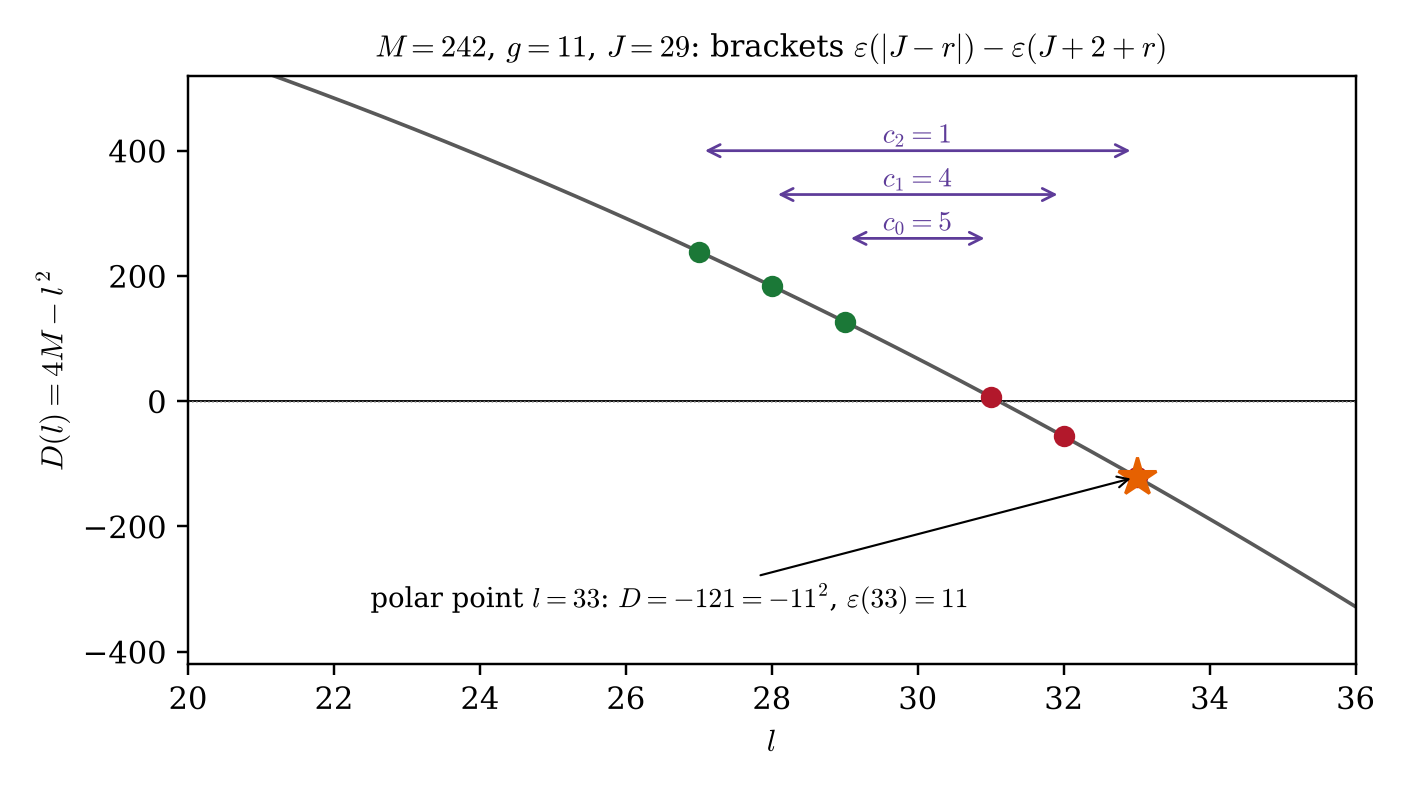
\includegraphics[width=0.8\textwidth]{fig_pairing.png}
\caption{The pairing in the proof of Theorem~\ref{thm:C} for $M=242$, $g=11$, $J=29$. The green points $l=J,J-1,J-2$ are paired with the red points $l=J+2,J+3,J+4$; the arrows carry the weights $c_r$. The point $l=33$ lies at $D=-121=-11^2$ and carries the polar value $\varepsilon(33)=11$; against $l_1=31$, where $D=7$ and $t=2$, it attains the bound of Lemma~\ref{lem:polar}.}\label{fig:pairing}
\end{figure}

\begin{figure}[ht]
\centering
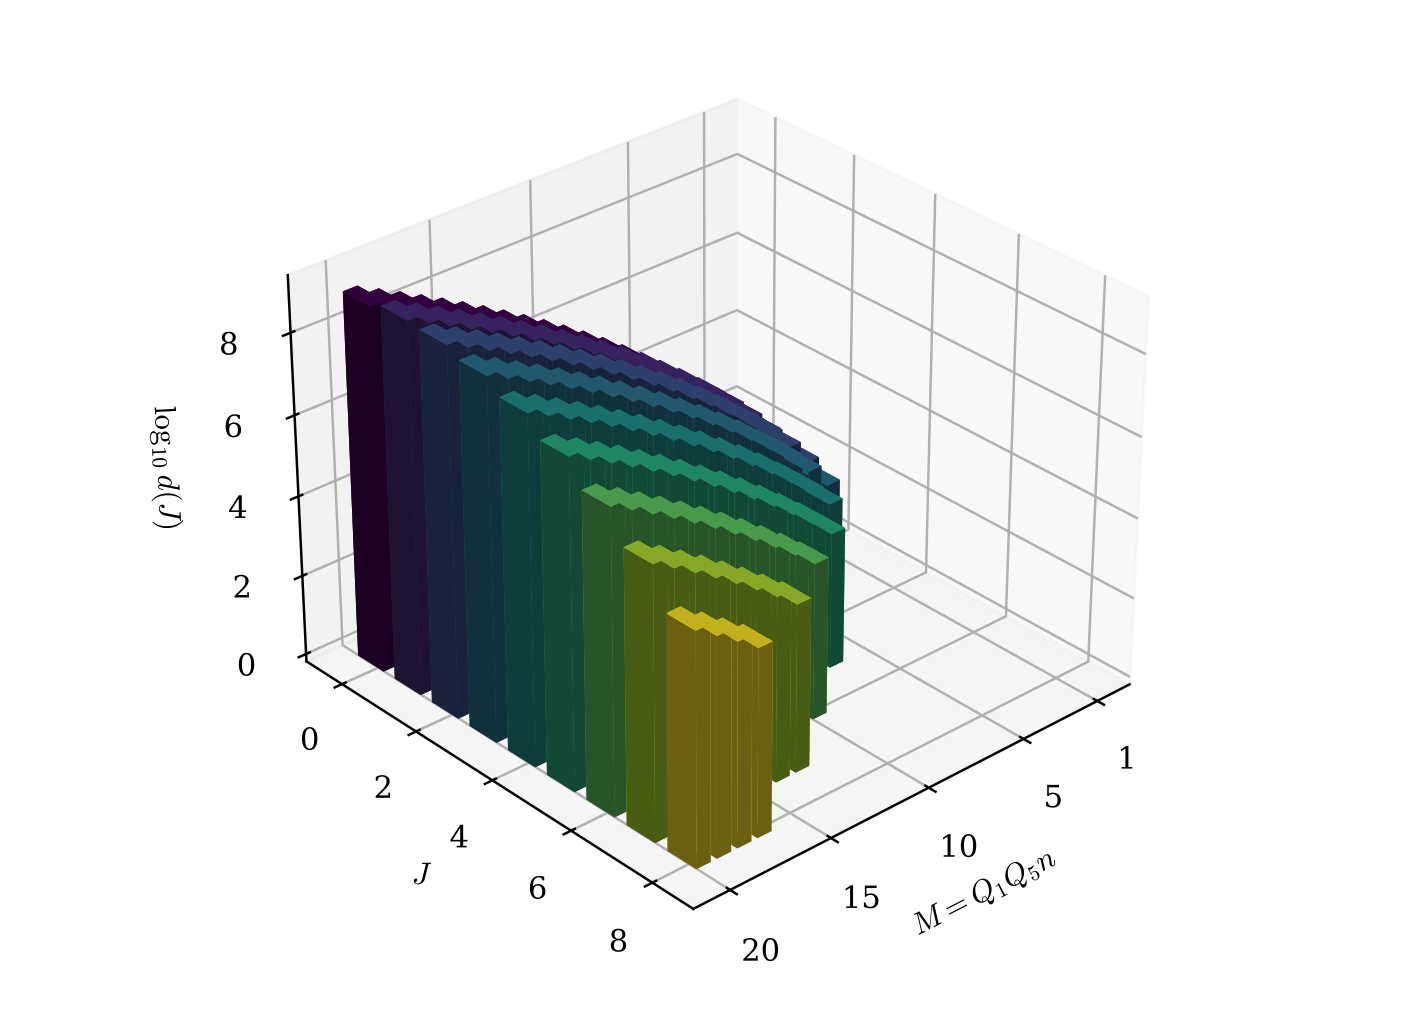
\includegraphics[width=0.74\textwidth]{fig_fixedJ.png}
\caption{The index $d(n,Q_1,Q_5,J)$ at fixed angular momentum for $g=\gcd(n,Q_1Q_5)=1$, $M=Q_1Q_5n\le20$ and all $J\ge0$ with $4M-J^2>0$, on a logarithmic scale.}\label{fig:fixedJ}
\end{figure}

\section{Remarks}\label{sec:remarks}

\subsection{Sharpness}
The divisor terms are exponentially smaller than the leading term for large discriminants: by Lemma~\ref{lem:aupper} the term $s=2$ of $W(D)$ is at most $e^{\frac\pi2\sqrt{D}(1+o(1))}$, while $\log|\cc(D)|=\pi\sqrt D\,(1+o(1))$ \cite[(2.7)]{Sen10}. The content of Proposition~\ref{prop:key} is that this separation already holds at the smallest discriminants, where it is tight: at $D=12$ the term $s=2$ takes $16$ of the $208$ units of the leading term in \eqref{eq:d4}, and $2W^*(12)$ is $42\%$ of $G(12)$. The polar values are smaller still, at most linear in the discriminant by Lemma~\ref{lem:polar}, but they are not negligible at small charges: the case $D_1=7$, $s_0=23$ of Lemma~\ref{lem:pair} uses more than half of $\varepsilon(l_1)=39$. The lower bound of Lemma~\ref{lem:alower} grows like $e^{2\sqrt6\sqrt n}$ instead of the true $e^{2\pi\sqrt n}$, which is why the analytic argument starts only at $k=\Kzero$.

\subsection{The U-duality invariant extension}
For charges with $\gcd(Q_1,Q_5,n)=1$, Maldacena, Moore and Strominger proposed the U-duality invariant extension of \eqref{eq:F} in which the divisor $s$ carries the weight $N(s)\,s$, with $N(s)$ the number of common divisors of $n,Q_1,Q_5,s,nQ_1/s,nQ_5/s,Q_1Q_5/s,nQ_1Q_5/s^2$, the sum running over the $s$ for which $l/s$ and all these quotients are integers \cite[(6.2)--(6.3)]{MMS99}. For such charges $N(s)=1$, since a common divisor of $n,Q_1,Q_5$ is $1$, so the weights again lie in $\{0,s\}$, are even in $l$, and are supported on divisors $s$ of $l$ with $s^2\mid M$. The proofs of Lemmas~\ref{lem:eps}, \ref{lem:polar} and~\ref{lem:pair} use nothing else: in Lemma~\ref{lem:eps}(2) the value at $D(l)=0$ becomes $2\sum s$ over a set of divisors of $l$, which is at most $2\sigma(l)\le l(l+1)$, and the bound $l_2\le\frac14(D_1+4)$ is unchanged. Hence, if the extension holds, the indices it predicts satisfy Theorems~\ref{thm:B} and~\ref{thm:C} for every charge with $\gcd(Q_1,Q_5,n)=1$.

\subsection{Charges of higher torsion}\label{ssec:torsion}
For four-dimensional charges with $\gcd(\ell_1,\ell_2)>1$ no formula for the index has been established \cite[\S2]{Sen10}, and the theorems say nothing about them. Corollary~\ref{cor:principle} reduces their positivity to a structural statement: any index of the form $(-1)^{\Delta+1}\sum_{s^2\mid\Delta}w(s)\,\cc(\Delta/s^2)$ with $w(1)=1$ and $|w(s)|\le s^2$ is positive, whatever the signs of the other weights. Any future formula of this shape, with the divisor weights bounded by $s^2$, would therefore give positive indices at once.\footnote{Sen remarks that the condition $\gcd(\ell_1,\ell_2)=1$ might be relaxed with the results of \cite{SSY06} for non-primitive charge vectors \cite[\S2]{Sen10}; no such formula has been derived.}

\section*{Declarations}

\subsection*{Data availability}
All data that support the findings of this study are contained in the article: Table~\ref{tab:a} lists the numbers $a(n)$ used in the finite part of the proof, and Appendix~\ref{app:finite} describes the verification. The program that repeats the verification, computes the tables and draws the figures is archived at doi:\zenodoCodeDOI.

\subsection*{Funding}
None.

\subsection*{Conflict of interest}
None.

\subsection*{Ethics statement}
This study involves no human participants, animals or personal data; no ethical approval was required.

\appendix

\section{Elementary facts}\label{app:standard}

\subsection*{Lagrange's identity}
For vectors $a,b,c,e\in\mathbb R^N$,
\[
(a\cdot c)(b\cdot e)-(a\cdot e)(b\cdot c)=\sum_{i<j}(a_ib_j-a_jb_i)(c_ie_j-c_je_i).
\]
Both sides are bilinear in $(a,b)$ and in $(c,e)$, so it suffices to take basis vectors $a=e_p$, $b=e_q$, $c=e_r$, $e=e_s$. The left side is $\delta_{pr}\delta_{qs}-\delta_{ps}\delta_{qr}$. On the right, the term $i<j$ is nonzero only if $\{p,q\}=\{i,j\}=\{r,s\}$ with $p\ne q$, and it is then $+1$ if $(p,q)=(r,s)$ and $-1$ if $(p,q)=(s,r)$. The two sides agree. In Lemma~\ref{lem:arith} this is applied with $a=Q$, $b=P$, $c=LQ$, $e=LP$, using $Q\cdot LP=P\cdot LQ$ because $L$ is symmetric.

\subsection*{Two inequalities}
For $0\le y\le\frac12$, the function $f(y)=\log(1-y)+y+y^2$ has $f(0)=0$ and $f'(y)=\frac{y(1-2y)}{1-y}\ge0$, so $\log(1-y)\ge-y-y^2$. For $m\ge1$ the divisors of $m$ are distinct elements of $\{1,\dots,m\}$, so $\sigma(m)\le1+2+\dots+m=\frac12m(m+1)$.

\subsection*{Jacobi's triple product}
For $|q|<1$ and $x\ne0$,
\[
\prod_{n\ge1}(1-q^{2n})(1+xq^{2n-1})(1+x^{-1}q^{2n-1})=\sum_{m\in\ZZ}x^mq^{m^2}
\]
\cite[Thm.~2.8]{And84}. Replace $q$ by $q^{1/2}$ and $x$ by $-\zeta q^{1/2}$. With $r=m+\frac12$ the sum becomes
\[
\sum_m(-1)^m\zeta^mq^{(m^2+m)/2}=\zeta^{-1/2}q^{-1/8}\sum_{r\in\ZZ+\frac12}(-1)^{r-\frac12}q^{r^2/2}\zeta^r=i\,\zeta^{-1/2}q^{-1/8}\vt_1(\tau,z).
\] The product becomes $\prod_n(1-q^n)(1-\zeta q^n)(1-\zeta^{-1}q^{n-1})=(1-\zeta^{-1})\prod_n(1-q^n)(1-\zeta q^n)(1-\zeta^{-1}q^n)$. Since $\zeta^{1/2}(1-\zeta^{-1})=\zeta^{1/2}-\zeta^{-1/2}$, this gives \eqref{eq:triple}, and squaring and dividing by $\eta^6=q^{1/4}\prod(1-q^n)^6$ gives \eqref{eq:product}.

\subsection*{A bound for $a(n)$ without modular forms}
For $u>0$,
\[
\log P(e^{-u})=6\sum_{m\ge1}\sum_{r\ge1}\frac{e^{-umr}}{r}=6\sum_{r\ge1}\frac1r\cdot\frac{e^{-ur}}{1-e^{-ur}}\le6\sum_{r\ge1}\frac{1}{ur^2}=\frac{\pi^2}{u},
\]
because $e^{-v}/(1-e^{-v})=1/(e^v-1)\le1/v$. Hence $a(n)\le e^{nu}P(e^{-u})\le e^{nu+\pi^2/u}$, and the choice $u=\pi/\sqrt n$ gives $a(n)\le e^{2\pi\sqrt n}$, the second bound of Lemma~\ref{lem:aupper}.

\section{The finite range}\label{app:finite}

The inequalities \eqref{eq:keya} and \eqref{eq:keyb} for $3\le D\le358$ involve integers only, and their verification consists of four steps.
\begin{enumerate}
\item[(F1)] The numbers $a(n)$, $0\le n\le\Kzero$, are computed from the recursion $n\,a(n)=6\sum_{i=1}^n\sigma(i)a(n-i)$ of Lemma~\ref{lem:alower}, or equivalently by multiplying out six copies of $\prod(1-q^n)^{-1}$; they are listed in Table~\ref{tab:a}.
\item[(F2)] For $-1\le E\le 358$, $|\cc(E)|$ is computed from \eqref{eq:theta}.
\item[(F3)] For $1\le E\le358$, $W(E)$ is computed from its definition, and $W^*(D)$ as a running maximum.
\item[(F4)] For each $D$ in the range with $D\equiv0,3\pmod 4$, the integers $G(D)$, $2W^*(D)$ and $16G(D)-16W^*(D)-(D+4)(D+8)$ are compared.
\end{enumerate}
Table~\ref{tab:key} lists the quantities for $D\le63$; the margin grows rapidly, as Figure~\ref{fig:margins} shows. The same program checks, as controls that the proofs do not use: the formula \eqref{eq:theta} against the direct expansion of $-\vt_1^2/\eta^6$ up to $q^{30}$ and against the product \eqref{eq:product} up to $q^{12}$; the bounds of Section~\ref{sec:a} for $n\le605$; the conclusions of Theorems~\ref{thm:A} to~\ref{thm:C} by evaluating \eqref{eq:d4}, \eqref{eq:d5} and \eqref{eq:drot} directly on $1722$ four-dimensional charges in Sen's normal form and $5750$ five-dimensional charges; all $868$ five-dimensional charges with $M\le600$ in which a polar value enters, together with the bound of Lemma~\ref{lem:polar}; and $3195$ charges for the extension of \cite{MMS99}.

\begin{table}[H]\centering\footnotesize
\caption{The numbers $a(n)$ of partitions of $n$ into parts of six colours, $0\le n\le 90$.}\label{tab:a}
\begin{tabular}{@{}rr@{\qquad}rr@{\qquad}rr@{}}\toprule
$n$ & $a(n)$ & $n$ & $a(n)$ & $n$ & $a(n)$\\\midrule
0 & 1 & 31 & 30227301468 & 62 & 13799370667455450\\
1 & 6 & 32 & 49522366656 & 63 & 19845194082605218\\
2 & 27 & 33 & 80590617278 & 64 & 28465163415636075\\
3 & 98 & 34 & 130307480730 & 65 & 40724826208003224\\
4 & 315 & 35 & 209396014650 & 66 & 58118725494437321\\
5 & 918 & 36 & 334492740175 & 67 & 82738453811650308\\
6 & 2492 & 37 & 531278722086 & 68 & 117504789092547003\\
7 & 6372 & 38 & 839204245278 & 69 & 166487707267085750\\
8 & 15525 & 39 & 1318587244800 & 70 & 235346673673043703\\
9 & 36280 & 40 & 2061234013149 & 71 & 331935256651796730\\
10 & 81816 & 41 & 3206265612102 & 72 & 467129825087621531\\
11 & 178794 & 42 & 4963610011174 & 73 & 655963278944277444\\
12 & 380051 & 43 & 7648740634158 & 74 & 919173274601444100\\
13 & 788004 & 44 & 11733857681850 & 75 & 1285312714955089064\\
14 & 1597725 & 45 & 17923026108974 & 76 & 1793621662235878482\\
15 & 3174210 & 46 & 27262103713383 & 77 & 2497928656596353478\\
16 & 6190182 & 47 & 41299026921900 & 78 & 3471941462435113530\\
17 & 11867310 & 48 & 62316761884412 & 79 & 4816410159748817880\\
18 & 22395359 & 49 & 93670787579400 & 80 & 6668809352618868378\\
19 & 41650050 & 50 & 140276509484724 & 81 & 9216404411744168100\\
20 & 76413078 & 51 & 209311092717496 & 82 & 12713856676088969832\\
21 & 138421358 & 52 & 311221082489247 & 83 & 17506907536752046098\\
22 & 247783113 & 53 & 461164908282750 & 84 & 24064191719868828650\\
23 & 438616728 & 54 & 681072218736560 & 85 & 33019905786901987212\\
24 & 768291650 & 55 & 1002575819281092 & 86 & 45230951219325322689\\
25 & 1332444330 & 56 & 1471174898831406 & 87 & 61853350983484206818\\
26 & 2289213495 & 57 & 2152131323752182 & 88 & 84444293827166272965\\
27 & 3898064226 & 58 & 3138799331684016 & 89 & 115098208842781661400\\
28 & 6581591157 & 59 & 4564363803456240 & 90 & 156627966849287037846\\
29 & 11023247880 & 60 & 6618341988415724 &  & \\
30 & 18320981569 & 61 & 9569726912844018 &  & \\
\bottomrule\end{tabular}\end{table}
\begin{table}[H]\centering\footnotesize
\caption{The quantities of Proposition~\ref{prop:key} for $3\le D\le 63$.}\label{tab:key}
\begin{tabular}{@{}rrrrr@{\qquad}rrrrr@{}}\toprule
$D$ & $|\hat c(D)|$ & $G(D)$ & $W(D)$ & $W^*(D)$ & $D$ & $|\hat c(D)|$ & $G(D)$ & $W(D)$ & $W^*(D)$\\\midrule
3 & 8 & 7 & 0 & 0 & 35 & 69168 & 40269 & 0 & 224\\
4 & 12 & 10 & 0 & 0 & 36 & 85500 & 49412 & 108 & 224\\
7 & 39 & 31 & 0 & 0 & 39 & 159372 & 90204 & 0 & 224\\
8 & 56 & 44 & 0 & 0 & 40 & 195312 & 109812 & 0 & 224\\
11 & 152 & 113 & 0 & 0 & 43 & 355224 & 195852 & 0 & 224\\
12 & 208 & 152 & 32 & 32 & 44 & 431984 & 236672 & 608 & 608\\
15 & 513 & 361 & 0 & 32 & 47 & 768885 & 413661 & 0 & 608\\
16 & 684 & 476 & 48 & 48 & 48 & 928720 & 496736 & 960 & 960\\
19 & 1560 & 1047 & 0 & 48 & 51 & 1621296 & 852411 & 0 & 960\\
20 & 2032 & 1348 & 0 & 48 & 52 & 1946352 & 1017632 & 0 & 960\\
23 & 4382 & 2822 & 0 & 48 & 55 & 3339201 & 1717905 & 0 & 960\\
24 & 5616 & 3584 & 0 & 48 & 56 & 3986656 & 2040304 & 0 & 960\\
27 & 11552 & 7170 & 72 & 72 & 59 & 6732232 & 3393031 & 0 & 960\\
28 & 14592 & 8976 & 156 & 156 & 60 & 7997184 & 4010528 & 2052 & 2052\\
31 & 28899 & 17347 & 0 & 156 & 63 & 13311450 & 6579218 & 351 & 2052\\
32 & 36088 & 21496 & 224 & 224 &  & & & & \\
\bottomrule\end{tabular}\end{table}

\begin{thebibliography}{99}

\bibitem{And84} G.~E.~Andrews, \emph{The Theory of Partitions}, Encyclopedia of Mathematics and its Applications \textbf{2}, Cambridge University Press, Cambridge, 1984. doi:10.1017/CBO9780511608650

\bibitem{Apo90} T.~M.~Apostol, \emph{Modular Functions and Dirichlet Series in Number Theory}, 2nd ed., Graduate Texts in Mathematics \textbf{41}, Springer, New York, 1990. doi:10.1007/978-1-4612-0999-7

\bibitem{BK97} C.~Bachas, E.~Kiritsis, \emph{$F^4$ terms in $N=4$ string vacua}, Nucl. Phys. B Proc. Suppl. \textbf{55} (1997), 194--199. doi:10.1016/S0920-5632(97)00079-0

\bibitem{BFKOV98} C.~Bachas, C.~Fabre, E.~Kiritsis, N.~A.~Obers, P.~Vanhove, \emph{Heterotic/type-I duality and D-brane instantons}, Nucl. Phys. B \textbf{509} (1998), 33--52. doi:10.1016/S0550-3213(97)00639-1

\bibitem{Bha22} D.~Bhattacharjee, \emph{Generalization of quartic and quintic Calabi--Yau manifolds fibered by polarized K3 surfaces}, Research Square (2022). doi:10.21203/rs.3.rs-1965255/v1

\bibitem{BN26} D.~Bhattacharjee, P.~Nandi, \emph{Enriques and Kummer surfaces arising from K3 involutions}, Preprints (2026). doi:10.20944/preprints202602.0098.v1

\bibitem{BMPV97} J.~C.~Breckenridge, R.~C.~Myers, A.~W.~Peet, C.~Vafa, \emph{D-branes and spinning black holes}, Phys. Lett. B \textbf{391} (1997), 93--98. doi:10.1016/S0370-2693(96)01460-8

\bibitem{BM13} K.~Bringmann, S.~Murthy, \emph{On the positivity of black hole degeneracies in string theory}, Commun. Number Theory Phys. \textbf{7} (2013), 15--56. doi:10.4310/CNTP.2013.v7.n1.a2

\bibitem{CGMS14} A.~Chowdhury, R.~S.~Garavuso, S.~Mondal, A.~Sen, \emph{BPS state counting in $\mathcal N=8$ supersymmetric string theory for pure D-brane configurations}, J. High Energy Phys. \textbf{2014}, no.~10 (2014), 186. doi:10.1007/JHEP10(2014)186

\bibitem{CGMS16} A.~Chowdhury, R.~S.~Garavuso, S.~Mondal, A.~Sen, \emph{Do all BPS black hole microstates carry zero angular momentum?}, J. High Energy Phys. \textbf{2016}, no.~4 (2016), 082. doi:10.1007/JHEP04(2016)082

\bibitem{CM24} A.~Chowdhury, S.~Maji, \emph{Counting $\mathcal N=8$ black holes as algebraic varieties}, J. High Energy Phys. \textbf{2024}, no.~5 (2024), 091. doi:10.1007/JHEP05(2024)091

\bibitem{CJ79} E.~Cremmer, B.~Julia, \emph{The $SO(8)$ supergravity}, Nucl. Phys. B \textbf{159} (1979), 141--212. doi:10.1016/0550-3213(79)90331-6

\bibitem{DGM11} A.~Dabholkar, J.~Gomes, S.~Murthy, \emph{Quantum black holes, localization and the topological string}, J. High Energy Phys. \textbf{2011}, no.~6 (2011), 019. doi:10.1007/JHEP06(2011)019

\bibitem{DGMS11} A.~Dabholkar, J.~Gomes, S.~Murthy, A.~Sen, \emph{Supersymmetric index from black hole entropy}, J. High Energy Phys. \textbf{2011}, no.~4 (2011), 034. doi:10.1007/JHEP04(2011)034

\bibitem{DMVV97} R.~Dijkgraaf, G.~Moore, E.~Verlinde, H.~Verlinde, \emph{Elliptic genera of symmetric products and second quantized strings}, Commun. Math. Phys. \textbf{185} (1997), 197--209. doi:10.1007/s002200050087

\bibitem{EZ85} M.~Eichler, D.~Zagier, \emph{The Theory of Jacobi Forms}, Progress in Mathematics \textbf{55}, Birkh\"auser, Boston, 1985. doi:10.1007/978-1-4684-9162-3

\bibitem{GSY06} D.~Gaiotto, A.~Strominger, X.~Yin, \emph{New connections between 4D and 5D black holes}, J. High Energy Phys. \textbf{2006}, no.~2 (2006), 024. doi:10.1088/1126-6708/2006/02/024

\bibitem{HR18} G.~H.~Hardy, S.~Ramanujan, \emph{Asymptotic formulae in combinatory analysis}, Proc. London Math. Soc. (2) \textbf{17} (1918), 75--115. doi:10.1112/plms/s2-17.1.75

\bibitem{KK96} R.~Kallosh, B.~Kol, \emph{$E_7$ symmetric area of the black hole horizon}, Phys. Rev. D \textbf{53} (1996), R5344--R5348. doi:10.1103/PhysRevD.53.R5344

\bibitem{KO97} E.~Kiritsis, N.~A.~Obers, \emph{Heterotic/type-I duality in $D<10$ dimensions, threshold corrections and D-instantons}, J. High Energy Phys. \textbf{1997}, no.~10 (1997), 004. doi:10.1088/1126-6708/1997/10/004

\bibitem{MMS99} J.~Maldacena, G.~Moore, A.~Strominger, \emph{Counting BPS black holes in toroidal type II string theory}, arXiv:hep-th/9903163 (1999).

\bibitem{Rad43} H.~Rademacher, \emph{On the expansion of the partition function in a series}, Ann. of Math. (2) \textbf{44} (1943), 416--422. doi:10.2307/1968973

\bibitem{Rad73} H.~Rademacher, \emph{Topics in Analytic Number Theory}, Grundlehren der mathematischen Wissenschaften \textbf{169}, Springer, Berlin, 1973. doi:10.1007/978-3-642-80615-5

\bibitem{Rob55} H.~Robbins, \emph{A remark on Stirling's formula}, Amer. Math. Monthly \textbf{62} (1955), 26--29. doi:10.2307/2308012

\bibitem{SBBT26} R.~Sadhu, D.~Bhattacharjee, S.~Bhattacharya, S.~N.~Thakur, \emph{$E_8\times E_8$ heterotic gravity and M-theory}, SSRN (2026). doi:10.2139/ssrn.6326718

\bibitem{Sen08r} A.~Sen, \emph{Black hole entropy function, attractors and precision counting of microstates}, Gen. Relativ. Gravit. \textbf{40} (2008), 2249--2431. doi:10.1007/s10714-008-0626-4

\bibitem{Sen08b} A.~Sen, \emph{$\mathcal N=8$ dyon partition function and walls of marginal stability}, J. High Energy Phys. \textbf{2008}, no.~7 (2008), 118. doi:10.1088/1126-6708/2008/07/118

\bibitem{Sen09a} A.~Sen, \emph{Quantum entropy function from $AdS_2/CFT_1$ correspondence}, Int. J. Mod. Phys. A \textbf{24} (2009), 4225--4244. doi:10.1142/S0217751X09045893

\bibitem{Sen09b} A.~Sen, \emph{Arithmetic of quantum entropy function}, J. High Energy Phys. \textbf{2009}, no.~8 (2009), 068. doi:10.1088/1126-6708/2009/08/068

\bibitem{Sen10} A.~Sen, \emph{Arithmetic of $\mathcal N=8$ black holes}, J. High Energy Phys. \textbf{2010}, no.~2 (2010), 090. doi:10.1007/JHEP02(2010)090

\bibitem{Sen11} A.~Sen, \emph{How do black holes predict the sign of the Fourier coefficients of Siegel modular forms?}, Gen. Relativ. Gravit. \textbf{43} (2011), 2171--2183. doi:10.1007/s10714-011-1175-9

\bibitem{Sen12} A.~Sen, \emph{Logarithmic corrections to rotating extremal black hole entropy in four and five dimensions}, Gen. Relativ. Gravit. \textbf{44} (2012), 1947--1991. doi:10.1007/s10714-012-1373-0

\bibitem{SSY06} D.~Shih, A.~Strominger, X.~Yin, \emph{Counting dyons in $\mathcal N=8$ string theory}, J. High Energy Phys. \textbf{2006}, no.~6 (2006), 037. doi:10.1088/1126-6708/2006/06/037

\bibitem{SV96} A.~Strominger, C.~Vafa, \emph{Microscopic origin of the Bekenstein--Hawking entropy}, Phys. Lett. B \textbf{379} (1996), 99--104. doi:10.1016/0370-2693(96)00345-0

\end{thebibliography}

\end{document}
